% ******************************* PhD Thesis Template **************************
% Please have a look at the README.md file for info on how to use the template

\documentclass[a4paper,times,numbered,print,index,oneside,PageStyleII,parskip=full]{Classes/PhDThesisPSnPDF}

% ******************************************************************************
% ******************************* Class Options ********************************
% *********************** See README for more details **************************
% ******************************************************************************

% `a4paper'(The University of Cambridge PhD thesis guidelines recommends a page
% size a4 - default option) or `a5paper': A5 Paper size is also allowed as per
% the Cambridge University Engineering Deparment guidelines for PhD thesis
%
% `11pt' or `12pt'(default): Font Size 10pt is NOT recommended by the University
% guidelines
%
% `oneside' or `twoside'(default): Printing double side (twoside) or single
% side.
%
% `print': Use `print' for print version with appropriate margins and page
% layout. Leaving the options field blank will activate Online version.
%
% `index': For index at the end of the thesis
%
% `draft': For draft mode without loading any images (same as draft in book)
%
% `abstract': To generate only the title page and abstract page with
% dissertation title and name, to submit to the Student Registry
%
% ************************* Custom Page Margins ********************************
%
% `custommargin`: Use `custommargin' in options to activate custom page margins,
% which can be defined in the preamble.tex. Custom margin will override
% print/online margin setup.
%
% *********************** Choosing the Fonts in Class Options ******************
%
% `times' : Times font with math support. ( The Cambridge University guidelines
% recommend using times)
%
% `fourier': Utopia Font with Fourier Math font
%
% `customfont': Use `customfont' option in the document class and load the
% package in the preamble.tex
%
% default or leave empty: `Latin Modern' font will be loaded.
%
% ********************** Choosing the Bibliography style ***********************
%
% `authoryear': For author-year citation eg., Krishna (2013)
%
% `numbered': (Default Option) For numbered and sorted citation e.g., [1,5,2]
%
% `custombib': Define your own bibliography style in the `preamble.tex' file.
% `\RequirePackage[square, sort, numbers, authoryear]{natbib}'
%
% **************************** Choosing the Page Style *************************
%
% `default (leave empty)': For Page Numbers in Header (Left Even, Right Odd) and
% Chapter Name in Header (Right Even) and Section Name (Left Odd). Blank Footer.
%
% `PageStyleI': Chapter Name next & Page Number on Even Side (Left Even).
% Section Name & Page Number in Header on Odd Side (Right Odd). Footer is empty.
%
% `PageStyleII': Chapter Name on Even Side (Left Even) in Header. Section Number
% and Section Name in Header on Odd Side (Right Odd). Page numbering in footer


% ********************************** Preamble **********************************
% Preamble: Contains packages and user-defined commands and settings
% ******************************************************************************
% ****************************** Custom Margin *********************************

% Add `custommargin' in the document class options to use this section
% Set {innerside margin / outerside margin / topmargin / bottom margin}  and
% other page dimensions
\ifsetMargin
\else
    \RequirePackage[left=37mm,right=30mm,top=35mm,bottom=30mm]{geometry}
    \setFancyHdr % To apply fancy header after geometry package is loaded
\fi

\usepackage{parskip}

% *****************************************************************************
% ******************* Fonts (like different typewriter fonts etc.)*************

% Add `customfont' in the document class option to use this section
\ifsetFont
\else
    % Set your custom font here and use `customfont' in options. Leave empty to
    % load computer modern font (default LaTeX font).  
    \RequirePackage{libertine} 
\fi
\hyphenpenalty=10000
\exhyphenpenalty=10000

% *****************************************************************************
% *************************** Bibliography  and References ********************

%\usepackage{cleveref} %Referencing without need to explicitly state fig /table

% Add `custombib' in the document class option to use this section
\ifsetBib % True, Bibliography option is chosen in class options
\else % If custom bibliography style chosen then load bibstyle here
    \RequirePackage[square, sort, numbers, authoryear]{natbib} % CustomBib
\fi

% changes the default name `Bibliography` -> `References'
\renewcommand{\bibname}{References}

% *****************************************************************************
% *************** Changing the Visual Style of Chapter Headings ***************
% Uncomment the section below. Requires titlesec package.

%\RequirePackage{titlesec}
%\newcommand{\PreContentTitleFormat}{\titleformat{\chapter}[display]{\scshape\Large}
%{\Large\filleft{\chaptertitlename} \Huge\thechapter}
%{1ex}{}
%[\vspace{1ex}\titlerule]}
%\newcommand{\ContentTitleFormat}{\titleformat{\chapter}[display]{\scshape\huge}
%{\Large\filleft{\chaptertitlename} \Huge\thechapter}{1ex}
%{\titlerule\vspace{1ex}\filright}
%[\vspace{1ex}\titlerule]}
%\newcommand{\PostContentTitleFormat}{\PreContentTitleFormat}
%\PreContentTitleFormat


% *****************************************************************************
% **************************** Custom Packages ********************************
% *****************************************************************************


% ************************* Algorithms and Pseudocode **************************

%\usepackage{algpseudocode} 

% https://en.wikibooks.org/wiki/LaTeX/Source_Code_Listings#Style_definition
\usepackage{listings}

%\definecolor{mygreen}{rgb}{0,0.6,0}
%\definecolor{mygray}{rgb}{0.5,0.5,0.5}
%\definecolor{mymauve}{rgb}{0.58,0,0.82}

%\lstset{ %
%    belowcaptionskip=1\baselineskip,
%    breaklines=true,
%    frame=L,
%    xleftmargin=\parindent,
%    language=Python,
%    showstringspaces=false,
%    basicstyle=\footnotesize\ttfamily,
%    keywordstyle=\bfseries\color{green!40!black},
%    commentstyle=\itshape\color{purple!40!black},
%    identifierstyle=\color{blue},
%    stringstyle=\color{orange},
%}

\usepackage{minted}


% ********************Captions and Hyperreferencing / URL **********************

% Captions: This makes captions of figures use a boldfaced small font. 
%\RequirePackage[small,bf]{caption}

\RequirePackage[labelsep=space,tableposition=top]{caption}
\renewcommand{\figurename}{Fig.} %to support older versions of captions.sty

% ************************ Formatting / Footnote *******************************

%\usepackage[perpage]{footmisc} %Range of footnote options 


% ****************************** Line Numbers **********************************

%\RequirePackage{lineno}
%\linenumbers

% ************************** Graphics and figures *****************************

%\usepackage{rotating}
%\usepackage{wrapfig}
%\usepackage{float}
\usepackage{subfig} %note: subfig must be included after the `caption` package. 

\usepackage[pdftex]{graphicx}
\newcommand{\HRule}{\rule{\linewidth}{0.5mm}}

% ********************************* Table **************************************

%\usepackage{longtable}
%\usepackage{multicol}
%\usepackage{multirow}
%\usepackage{tabularx}


% ***************************** Math and SI Units ******************************

\usepackage{amsfonts}
\usepackage{amsmath}
\usepackage{amssymb}
%\usepackage{siunitx} % use this package module for SI units


% ******************************************************************************
% ************************* User Defined Commands ******************************
% ******************************************************************************

% *********** To change the name of Table of Contents / LOF and LOT ************

%\renewcommand{\contentsname}{My Table of Contents}
%\renewcommand{\listfigurename}{My List of Figures}
%\renewcommand{\listtablename}{My List of Tables}


% ********************** TOC depth and numbering depth *************************

\setcounter{secnumdepth}{2}
\setcounter{tocdepth}{2}

% ******************************* Nomenclature *********************************

% To change the name of the Nomenclature section, uncomment the following line

%\renewcommand{\nomname}{Symbols}


% ********************************* Appendix ***********************************

% The default value of both \appendixtocname and \appendixpagename is `Appendices'. These names can all be changed via: 

%\renewcommand{\appendixtocname}{List of appendices}

%\renewcommand{\appendixname}{Appndx}


% ************************ Thesis Information & Meta-data **********************
%% The title of the thesis
\title{Application of Machine Learning Techniques to Next Generation Sequencing Quality Control} 
%\texorpdfstring is used for PDF metadata. Usage:
%\texorpdfstring{LaTeX_Version}{PDF Version (non-latex)} eg.,
%\texorpdfstring{$sigma$}{sigma}

%% The full name of the author
\author{Sam Nicholls}

%% Department (eg. Department of Engineering, Maths, Physics)
\dept{Department of Computer Science}

%% University and Crest
\university{Aberystwyth University}
\crest{
\includegraphics[width=0.5\textwidth]{University_Crest}}

%% You can redefine the submission text:
% Default as per the University guidelines: This dissertation is submitted for
% the degree of Doctor of Philosophy
%\renewcommand{\submissiontext}{change the default text here if needed}

%% Full title of the Degree 
\degree{Computer Science and Statistics BSc}

%% College affiliation (optional)
\college{}

%% Submission date
\degreedate{2014}

%% Meta information
\subject{} \keywords{}



% ***************************** Abstract Separate ****************************** 
% To printout only the titlepage and the abstract with the PhD title and the 
% author name for submission to the Student Registry, use the abstract option in
% the document class. 

\ifdefineAbstract
 \includeonly{Abstract/abstract} 
\else
\fi


% ******************************** Front Matter ********************************
\begin{document}


\frontmatter

\begin{titlepage}
\begin{center}

% Upper part of the page. The '~' is needed because \\
% only works if a paragraph has started.

\includegraphics[width=0.2\textwidth]{University_Crest}~\\[1cm]

\textsc{\huge Aberystwyth University}\\
\textsc{Computer Science and Statistics (GG34)}\\
\textsc{\Large CS396: Minor Project}\\[1.5cm]

% Title
\HRule \\[0.4cm]
{ \huge \bfseries Application of Machine Learning Techniques to Next Generation Sequencing Quality Control \\[0.5cm] }
\HRule \\[1.5cm]

% Author and supervisor
\begin{minipage}{0.4\textwidth}
    \begin{flushleft} \large
        \emph{Author:}\\
        Sam Nicholls \small{msn}
    \end{flushleft}
\end{minipage}
\begin{minipage}{0.4\textwidth}
    \begin{flushright} \large
        \emph{Supervisor:} \\
        Dr.~Amanda Clare \small{afc}
    \end{flushright}
\end{minipage}


\vfill
% Bottom of the page
Draft\\
{\large \today}

\end{center}
\end{titlepage}

%TODO Wordcount includes declaration and abstract
%\include{Dedication/dedication}
% ******************************* Thesis Declaration ********************************
\begin{declaration}

I certify that except where indicated, all material in this thesis is the result
of my own investigation and references used in preparation of the text have been
cited. The work has not previously been submitted as part of any other assessed
module, or submitted for any other degree or diploma.

% Author and date will be inserted automatically from thesis.tex \author \degreedate

\end{declaration}

%% ************************** Thesis Acknowledgements *****************************
\begin{acknowledgements}

\end{acknowledgements}

%\begin{abstract}

Over the past few years advances in genetic sequencing hardware have introduced
the concept of massively parallel DNA sequencing, reducing both the time and cost
involved in performing genetic analysis. However, these
"next-generation" processes are complicated and open to error, thus
quality control is an essential step to assure confidence in any downstream
analyses carried out.

This project investigates the accuracy of a range of decision tree classifiers
for a series of quality control data sets and shows it is possible to
generate minimal yet accurate models, creating trees which closely resemble the
behaviour of an already existing QC system.

This project also introduces \textbf{Frontier}, a Python package which provides
users with interfaces for the reading, storage and retrieval of large machine
learning data sets; \textbf{Goldilocks}, a Python class which can be used
to find a region on a genome that expresses a desired density of variants across
different studies; and contributions to internal tools used as the Sanger
Institute and existing widely used open-source bioinformatics software.

\vskip 1.5cm
\textbf{Words} 15,999

\end{abstract}


% *********************** Adding TOC and List of Figures ***********************

\tableofcontents
%\listoffigures
%\listoftables

% \printnomenclature[space] space can be set as 2.5cm between symbol and
% description
%\printnomencl

% ******************************** Main Matter *********************************
\mainmatter

%******************************************************************************
\chapter{Introduction}
\ifpdf
    \graphicspath{{Chapter1/Figs/Raster/}{Chapter1/Figs/PDF/}{Chapter1/Figs/}}
\else
    \graphicspath{{Chapter1/Figs/Vector/}{Chapter1/Figs/}}
\fi

%%%%%%%%%%%%%%%%%%%%%%%%%%%%%%%%%%%%%%%%%%%%%%%%%%%%%%%%%%%%%%%%%%%%%%%%%%%%%%%

Over the past few years advances in genetic sequencing hardware have introduced
the concept of massively parallel DNA sequencing; allowing potentially billions
of chemical reactions to occur simultaneously, reducing both time and cost
required to perform genetic analysis\citep{HMG}. However, these
"next-generation" processes are complex and open to error\citep{Illumina}, thus
quality control is an essential step to assure confidence in any downstream
analyses performed.

%%%%%%%%%%%%%%%%%%%%%%%%%%%%%%%%%%%%%%%%%%%%%%%%%%%%%%%%%%%%%%%%%%%%%%%%%%%%%%%
\section{Project Aims}

The project consists of two sub-projects;

\begin{itemize}
    \item Analysis of a current quality control system in place
    \item Identification of quantifiable sample properties that affect downstream analysis
\end{itemize}


%TODO Samples or lanelets?
%TODO Github link in footnote rather than reference?
\subsection{Analysis of Current System}
% Lanes and lanelets have not been introduced yet and I think this works better
% as an introduction to the project rather than getting too heavy with
% terminology first.
With the support of the Wellcome Trust Sanger Institute in Cambridge, this
project works with the Human Genetics Informatics team to investigate
\textbf{auto\_qc}\citep{github:autoqc}, the institute's current automated quality control tool.

During genetic sequencing a large number of metrics are generated to determine
the quality of the data read from the sequencing hardware itself. As part of the
current vertebrate sequencing pipeline\citep{github:vr-pipe} at the institute,
\textbf{auto\_qc} is responsible for applying quality control to samples within
the pipeline by comparing a modest subset of these metrics to simple hard-coded
hard thresholds; determining whether a particular sample has reached a level that
requires a warning, or has exceeded the threshold and failed entirely. Whilst
this does catch most of the very poor quality outputs, a large number of samples
are flagged for manual inspection at the warning level; a time consuming task
which invites both inefficiency and error.

In practise most of these manual decisions are based on inspecting a range of
diagnostic plots which suggests that a machine learning classifier could
potentially be trained on the combinations of quality control statistics
available to make these conclusions without the need for much human
intervention\citep{marireport}.

The first part of the project aims to apply machine learning techniques to
replicate the current \textbf{auto\_qc} rule set by training a decision tree
classifier on a large set of these quality metrics. The idea is to investigate
whether these simple threshold based rules can be recovered from such data, or
whether a new classifier would produce different rules entirely. During this
analysis it is hoped the classifier may be able to identify currently unused
quality metrics that improve labelling accuracy. An investigation on the
possibility of aggregating or otherwise reducing the dimensions of some of the
more detailed quality statistics to create new parameters will also be
conducted.

The goal is to improve efficiency of quality control classification, whether by
improving accuracy of pass and fail predictions over the current system or
merely being able to provide additional information to a lab technician
inspecting samples labelled with a warning to reduce arbitrary decisions.

%%%%%%%%%%%%%%%%%%%%%%%%%%%%%%%%%%%%%%%%%%%%%%%%%%%%%%%%%%%%%%%%%%%%%%%%%%%%%%%
\subsection{Identification of Properties that affect Downstream Analysis}

The other half of this project is motivated by the question "What \textit{is}
good and bad in terms of quality?"

To be able to classify samples as a pass or a fail with understanding, we need
an idea of what actually constitutes a good or bad quality sample and must look
at the effects quality has on analysis performed downstream from sequencing.
An example of such is \textbf{variant calling} --- the process of identifying
differences between a DNA sample (such as your own) and a known reference
sequence.

%TODO Need to improve explanation here, don't like the simplification and feel
% it might just be hindering understanding of what we're doing
%TODO Difficult to discuss this without the word lanelets, samples vs.
% sub-samples isn't making as much sense as I'd like
%TODO Use a figure
Given two high quality data sources where DNA sequences from individuals were
identified in two different ways (one of which being next-generation sequencing)
it would be possible to measure the difference between each corresponding pair.
Using this, we could investigate the effect of leaving out part of the
next-generation sample during the variant calling process.
If we were to leave a part of a sample out of the variant calling
pipeline would the variants found be more (or less) accurate than if it had been
included? Would they agree more (or less) with the variants called after using
the non next-generation sequencing method?

Having identified such sub-samples, can quality control metrics from the
previous part be found in common? If so, such parameters would identify "good"
or "bad" samples straight out of the machine! Samples that exhibit these quality
variables will go on to improve or detriment analysis.


%%%%%%%%%%%%%%%%%%%%%%%%%%%%%%%%%%%%%%%%%%%%%%%%%%%%%%%%%%%%%%%%%%%%%%%%%%%%%%%
\section{Project Method}
\subsection{Methodology}

%TODO More coherant waffling needed
%TODO Explain CRACK customer?
%TODO Do I need to reference this section as my Assignment 3 report?
Clearly some team-based practices invited by agile methodologies ---
pair programming immediately comes to mind --- are not applicable in a solo
project. It is also unreasonable to expect an "on-site" customer for this
particular project. In \textit{The Case Against Extreme Programming}, Matt Stephens
describes a "self referential safety net" where the perceived traps in each
practice are supported and "made safe" by other XP practices.  This would seem
to rule out XP as a viable methodology for a solo-project as cutting out some
of the processes that allow this form of evolutionary design to work (and
flatten that cost-of-change curve) can introduce serious flaws to the
management of a project and potentially result in failure. In the same breath
it is important to remember that not all agile processes need be discarded just
because XP seems incompatible. Indeed, some processes seem like common sense,
for example; frequent refactoring, simple design, continuous integration and
version control. Test driven development could also prove a useful process to
consider as part of a methodology for this project, setting up a framework that
allows for quick and frequent testing (before coding) and ensuring that any
refactoring has a positive (or at least non-negative) effect on the system
could be a worthwhile contribution to efficiency.

Could a more plan driven approach or form of agile-plan hybrid be considered
appropriate here? In \textit{Balancing Agility and Discipline}, Boehm
and Turner introduce the idea of "homegrounds" for both agile and plan driven
approaches; I note here that for projects that require high reliability and
feature a non-collocated "CRACK customer" in fact align with some of these
homegrounds for plan driven development. Combined with the thought that the
project requirements will also be relatively stable it would seem that there
may be no reason to switch to a more agile methodology as its primary feature
is the welcoming of change that is not even needed? Perhaps this is the naivety
of an optimist!

%TODO Using I
%TODO Ring of Snakes probably needs elaboration
Personally I think I would approach this with a form of agile-plan hybrid; I
like the idea of quick iterations and getting feedback as opposed to leaving
acceptance testing until the very end of the project, but I also want a somewhat
detailed feedback process. Whilst through Neil Taylor's course \textit{Agile
Methodologies} it was suggested that it is dangerous to pick and choose
processes (don’t anger the Ring of Snakes!) and also merely paying "lip service"
to agile must be avoided (otherwise what's the point?), I feel that on this
occasion it can be justified by the size of the project itself.

%TODO Opportunity to drop the word pipeline and describe what it is for future
%use
This project will consist of many research steps, each requiring some form of
computational process to prepare the data for the next step. Whilst the
implementations of the algorithms themselves pose computational complexity,
there appears to be little challenge from a planning perspective and in fact a
looser overall plan should probably be considered as we must account for
unforseen and unexpected outcomes from each research step.

The most important part of ensuring this project stays on track will be the
development of a sensible testing methodology to ensure we are not only moving
in the right direction in terms of which algorithm and parameters to use but
also in terms of reliably measuring performance over time in a way that allows
justification of such design choices.

Despite this trail of thought, given the research grounding this project entails
it might be required to look beyond traditional and even modern software
development methodologies and investigate a more scientific approach. A simple
"scientific method" would involve establishing a null hypothesis that can be
proven false by testing (eg: "\textbf{auto\_qc} classifier is more
accurate than the new classifier") and executing experiments that
attempt to prove this null hypothesis false in favour of an alternative
hypothesis (typically the opposite, eg: "The new classifier is more
accurate than the old classifier"). This form of hypothesis testing
could essentially become the project's acceptance tests (providing we have an
empirical definition of what "more accurate" means in terms of this
system) and any modification can be classed as an experiment ("Do these
parameters allow us to reject the null hypothesis?").  Although care must be
taken not to let this descend into unstructured cycles of mere hack-and-test,
code-and-fix style programming.

Overall it is rather difficult to select a methodology for a project such as
this, the research element makes it almost impossible to draw on previous
personal experience for ideas of what development processes may or may not be
effective.

\subsection{Task and Time Management}
Shortly before embarking on this dissertation project, I had written my own todo
list web application; \textbf{Triage}\citep{github:triage}. This will be useful
in keeping track of current objectives and allow prioritisation. The list used to
organise my project is also publicly available\citep{sam:triage}.

\subsection{Time Considerations} It must be remembered that this project needs
to meet the requirements for a \textit{minor} project and is to be completed
alongside the study of several other modules which each have their own
assignments and obligations. It would be easy to become overly ambitious and
thus aims and goals will need to be revised as both obstacles and breakthroughs
are encountered.


% P1
%*****************************************************************************************
\part{Analysis of Current System}
\chapter{Introduction and Background}
\ifpdf
    \graphicspath{{Chapter2/Figs/Raster/}{Chapter2/Figs/PDF/}{Chapter2/Figs/}}
\else
    \graphicspath{{Chapter2/Figs/Vector/}{Chapter2/Figs/}}
\fi

%%%%%%%%%%%%%%%%%%%%%%%%%%%%%%%%%%%%%%%%%%%%%%%%%%%%%%%%%%%%%%%%%%%%%%%%%%%%%%%
\section{Introduction}

This part of the project can be outlined as follows:

\begin{itemize}
    \item Collect data sets on which a machine learning classifier is to be trained
    \item Construct a program capable of processing and storing such data sets
        such that required subsets of the data can be quickly and easily
        returned for further analysis
    \item Select a suitable machine learning framework to handle the training
        and validation of a classifier
    \item Ensure a robust validation methodology exists for assuring quality of
        our own results
    \item Set up an environment capable of allowing results from such a
        classifier to be stored and compared
    \item Training a suitable classifier on the collected data sets
    \item Perform experiments by selecting subsets of the variables and
        observations and measure whether classification accuracy is improved
\end{itemize}


%%%%%%%%%%%%%%%%%%%%%%%%%%%%%%%%%%%%%%%%%%%%%%%%%%%%%%%%%%%%%%%%%%%%%%%%%%%%%%%
\section{Concepts and Terminology}
\subsection{DNA and Bases}

...DNA is made up of four bases; G, C, T and A...


\subsection{Next Generation Sequencing}

...the process of recovering or extracting the sequence of nucleotide bases...


\subsection{Variants and SNPs}
...for the purpose of this study we are only interested in single nucleotide
polymorphisms (SNPs) "snips" ...

...their \textit{position} refers to the index of the base of the chromosome in
which the polymorphism exists...
...commonly these are 1-indexed (although this is not always the case) and thus
care must be taken to ensure this is accounted for at any step where positions
are considered...

...SNPs...

\textbf{variant calling} - the process of identifying bases in a sample that
differ from the reference genome (this is a little simple as you also need to
discern as whether the difference is actually a polymorphism or not).



\subsection{Samples, Lanes and Lanelets}
\label{chap:samplelanelanelets}

%TODO Draw a vector of the lanelets diagram
%TODO Illumina DNA Synthesis Image
A \textbf{sample} is a distinct DNA specimen extracted from a particular person.
For the purpose of sequencing, samples are pipetted in to a \textit{flowcell}
such as the one in Figure~\ref{fig:flowcell} -- a glass slide
containing a series of very thin tubules known as \textbf{lanes}.  It is
throughout these lanes that the chemical reactions involved in sequencing take place.

\begin{figure}[htbp!]
    \centering
    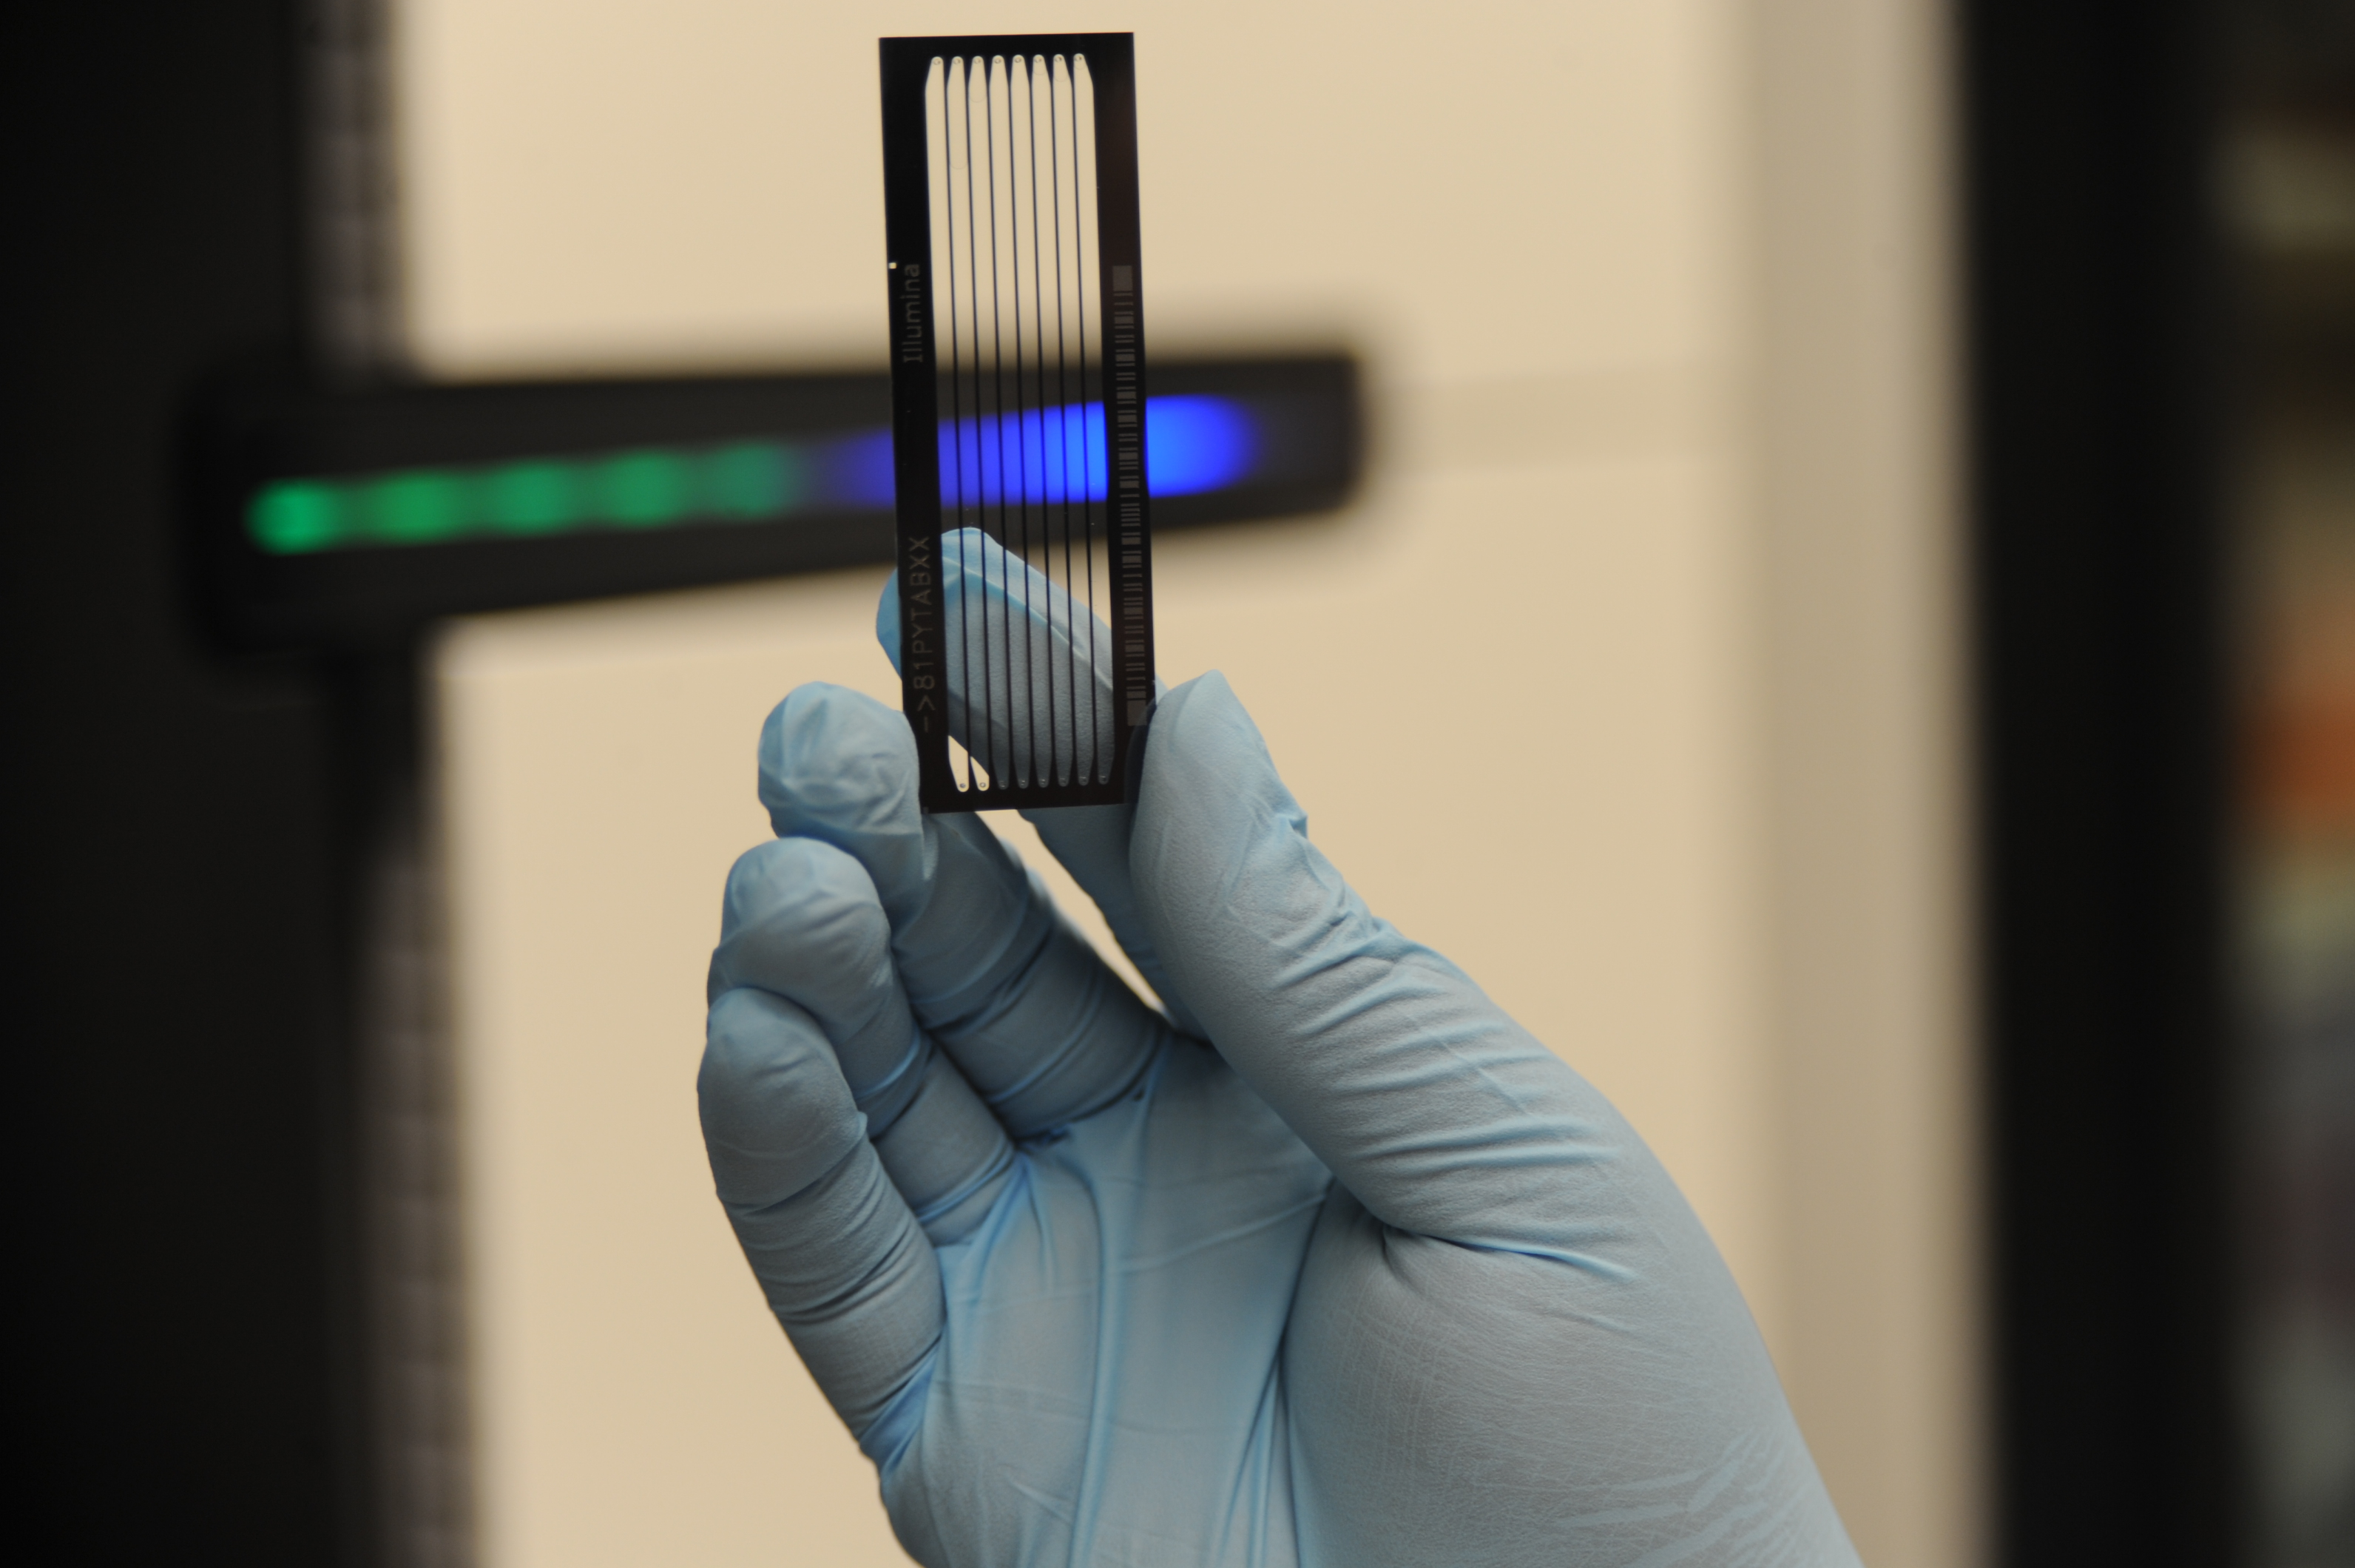
\includegraphics[width=0.4\textwidth]{NHGRI-80102}
    \caption[flowcell]{An Illumina HiSeq Flowcell\citep{img:flowcell}}
    \label{fig:flowcell}
\end{figure}

Once inserted, samples are amplified \textit{in situ}, in the flowcell itself. A
process in which the genetic material of each sample is caused to multiply in
magnitude to form a dense cluster of the sample around the original. Millions of
clusters will be created throughout each lane of the flowcell.

Note that a lane can contain more than one sample and a sample can appear in
more than one lane; this is known as \textit{sample multiplexing} and helps to
ensure that the failure of a particular lane does not hinder analysis of a
sample (as it will still be sequenced as part of another lane).

%TODO Describe lanelet as a Sanger coined term

The more abstract of the definitions, a \textbf{lanelet} is the aggregate read
of all clusters of a particular sample in a single lane.
Figure~\ref{fig:lanelets} attempts to highlight examples of a this (circled in
blue -- not all lanelets are highlighted). For example Lane 5 shows the four
clusters (in reality there would be millions) of Sample A combine to
represent a lanelet. A lane will have as many lanelets as it does samples.

%TODO Describe lanelet ID

\begin{figure}[htbp!]
    \centering
    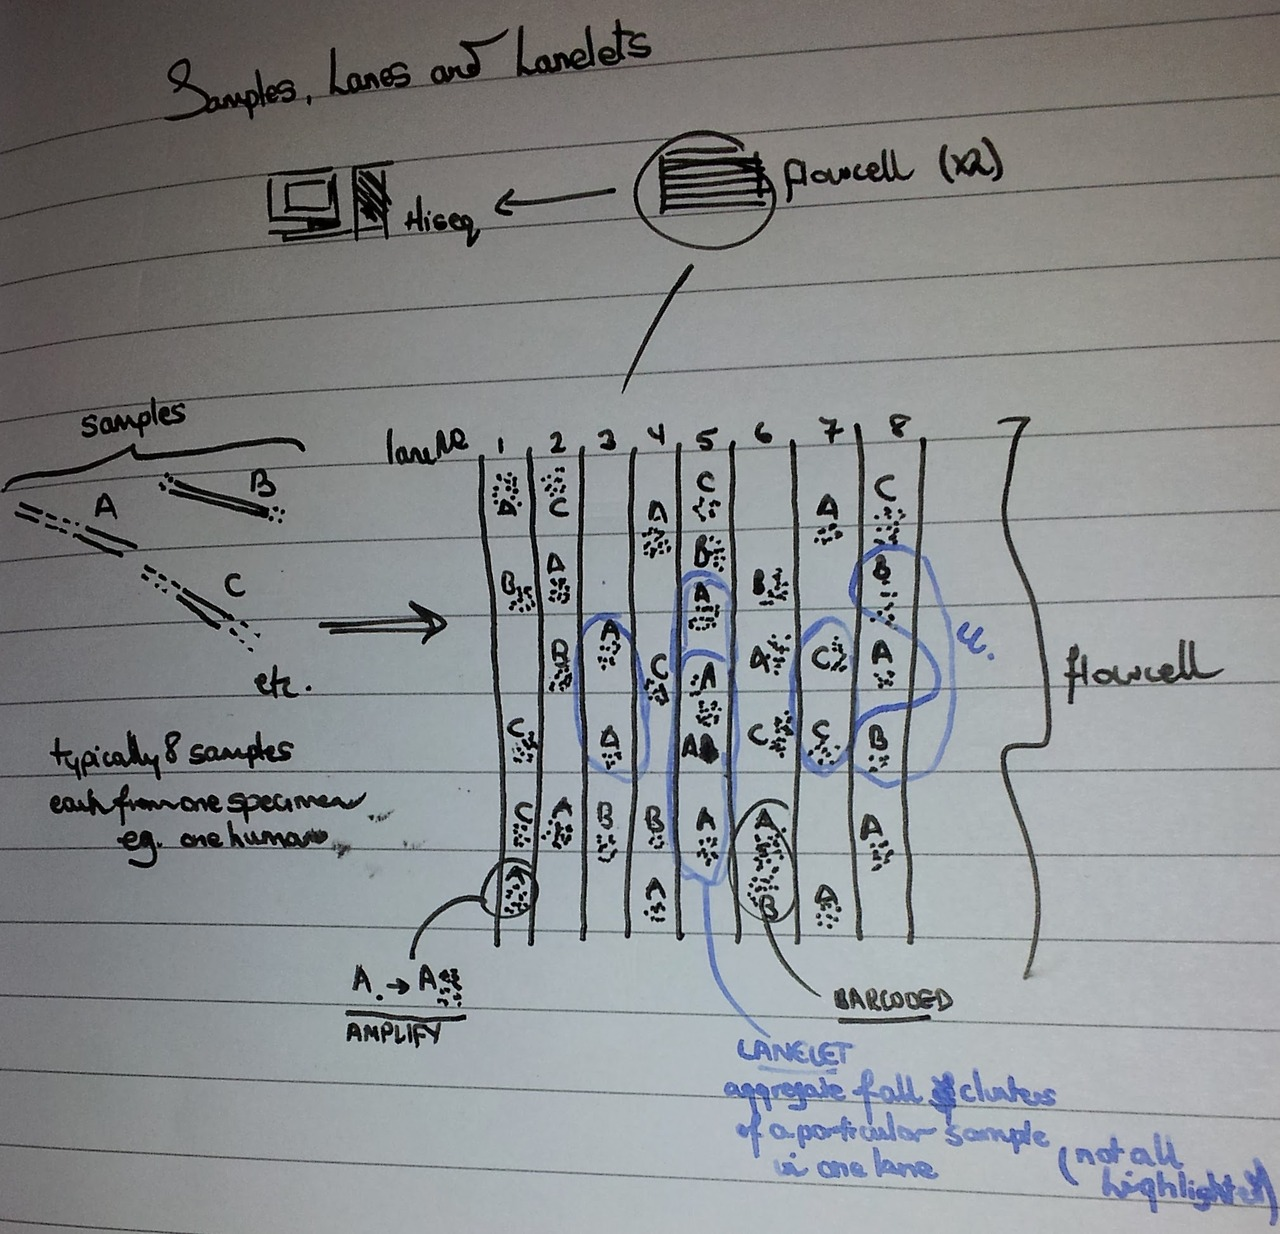
\includegraphics[width=0.5\textwidth]{lanelets}
    \caption[lanelets]{Example of flowcell with some lanelets highlighted}
    \label{fig:lanelets}
\end{figure}


%%%%%%%%%%%%%%%%%%%%%%%%%%%%%%%%%%%%%%%%%%%%%%%%%%%%%%%%%%%%%%%%%%%%%%%%%%%%%%%
\chapter{Materials and Methods}
\section{Input Data and Format}
\subsection{"BAMcheckR'd" Data}
\label{chap:bamcheckr-data}

%NOTE Assuming lanelets have been described by this point...
%TODO samtools stats actually generates this data rather than "the seq process"
As part of the project I have been granted access to significant data sets at the
Sanger Institute, unlocking quality control data for two of the largest studies
currently undergoing analysis. A wide array of quality metrics are available for
each and every lanelet that forms part of either of the two studies, totalling
13,455 files.
%TODO Cite and explain the security policy for this data

%9154 (68\%), 1542 (11\%), 2759 (21\%)...

%TODO Explain a BAM file
The files are created by \textbf{samtools stats} -- part of a collection of
widely used open-source utilities for post-processing and manipulation of large
alignments such as those produced by next-generation sequencers that are
released under the umbrella name of "SAMtools"\citep{samtools} (Sequence
Alignment and Map Tools). \textbf{samtools stats} collects statistics from
sequence data files and produces key-value summary numbers as well as more
complex tab delimited dataframes tabulating several metrics over time.

%TODO Was samtools stats known as bamcheck, or did it replace it?
The output of \textbf{samtools stats} is then parsed by an in-house tool called
\textbf{bamcheckr}\footnote{Named such as \textbf{samtools stats} now incorporates
\textbf{bamcheck} and the tool is written in R} which supplements the summary
numbers section of the \textbf{samtools stats} output with additional metrics
that are later used by \textbf{auto\_qc} for classification.  This process
appends additional key-value pairs in the summary numbers section.  A truncated
example of a "bamcheckr'd" file can be found in Appendix~\ref{app:bamcheckr}.

It is these summary numbers that will be the main focus of our learning task.


\subsection{auto\_qc Decision Data}

To use these "bamcheckr'd" files for training and testing a machine learning
classifier, it is necessary to map each file to a classification result from
\textbf{auto\_qc}. The one-to-one mapping between each input file and its label
are provided by the Sanger Institute in a separate file hereafter referred to as
the \textit{AQC Decision Matrix} or \textit{AQC (Decision) File}.

A truncated example of such a file can be found in
Appendix~\ref{app:aqc_matrix}.  Only the first few columns are included --
indeed we are only interested in the \textit{lanelet} and \textit{aqc} fields
which provide an identifier that maps the row to a given input file and its
classification by \textbf{auto\_qc} respectively.  Latter columns pertain to a
breakdown of decisions made by \textbf{auto\_qc} which are not included in the
example for confidentiality (and brevity).


%%%%%%%%%%%%%%%%%%%%%%%%%%%%%%%%%%%%%%%%%%%%%%%%%%%%%%%%%%%%%%%%%%%%%%%%%%%%%%%
\section{Development Environment}
\subsection{Language}
\label{part1:dev:lang}

%TODO Better opening
Python was selected for the language of the program designed to handle this vast
array of input data, more out of personal taste rather than a detailed analysis
of required performance and features. From previous experience I was happy with
the performance of Python when processing large datasets in terms of both
file handling operations and storing the data in memory for later use. Python's
generous choice of both built-in and third-party libraries have proven useful.
Due to its concise and flexible nature it is possible to rapidly
develop applications and its readability eases ongoing maintenance; useful given
the short time-span allocated for this project and the possibility of others
wishing to contribute to the project codebase after completion.

Whilst the choice was made primarily on preference, this is not to say other
options were not considered: a highly popular Java-based collection of data
mining tools, \textbf{WEKA}\citep{weka} would certainly have provided a
framework for building decision tree classifiers but did not
appear to offer any significant features that were unavailable elsewhere, whilst
Java itself has the added constraint of requiring a virtual machine to be
installed which could be undesirable from a performance or security
standpoint when the application is deployed to servers at the Sanger Institute.

%...although performance has improved considerably from previous Java versions\citep{Bouckaert}

Difficulty was also encountered finding example implementations for \textbf{WEKA}
with most documentation and tutorials providing information for performing
analysis via the graphical "Explorer" interface instead, which would not be
appropriate for quickly setting up and repeating experiments automatically.

Given the quality data we'll be using to train a machine learning classifier is
output from the previously mentioned R script, \textbf{bamcheckr}, it was worth
briefly investigating the options available for R itself as the potential of
integrating the learning and predicting functions right in to the same process
that outputs the data seemed convenient.

Whilst the \textbf{tree}\citep{man:rtree} and \textbf{rpart}\citep{man:rpart}
packages are available for constructing decision trees in R (and actually
\textbf{RWeka} provides an R interface to \textbf{WEKA}) neither appeared to be
as robust as other more well-known frameworks. Also putting it politely, the
programming paradigm of R\citep{man:R} is rather different to other languages
and can significantly increase development time (and frustration\citep{argh}) if
one is not well versed in the patterns and grammar of the language  and it
seemed best to stick to one's comfort zone given the brief timescale for the
project.

Had performance been a critical decision factor, lower level languages such as
C, C++ or even Fortran could be used. Briefly looking at frameworks available
for C++ in particular, two popular solutions include: \textbf{dlib}\citep{dlib},
which did not support tree-based classifiers but did offer implementations of
other potentially useful algorithms such as multi-class support vector machines;
and \textbf{Shark}\citep{shark}, which supported both decision tree and random
forest classifiers. Both packages also provided a series of utility functions
for performing mathematical or statistical operations on vectors of data.


\subsection{Framework}

Having studied the \textit{Machine and Intelligent Learning} module in my final
year, the prospect of getting stuck in to the deep of a machine learning
algorithm was exciting. However the reality is a lot of cumulative time and
effort has gone in to the creation and optimisation of a framework, which is
unlikely to be surpassed successfully by a short-term one-person project. Thus
utilisation of a third party machine learning library seems a wise investment
for the project's codebase.

There are clearly numerous machine learning frameworks available in many
languages, some of which were touched upon in the previous section and formed
part of the development environment decisions.
Whilst it is obviously unnecessary to select a framework which uses
the same language as the project, it seemed counter-intuitive to select otherwise,
for the establishing of additional arbitrary output and input steps to move data
between the two environments could impede prompt experiment repeatability and
introduce error.

A mixed bag of machine learning frameworks exist in Python\citep{py:for-ai},
ranging from several highly active general purpose libraries to a multitude of
smaller projects that focus on one specific learning task.

I investigate two of the larger libraries;
\textbf{scikit-learn}\citep{scikit-learn} and \textbf{Orange}\citep{orange},
primarily as their general purpose nature will allow exploration of various
classifier solutions (given time) without the need to integrate many packages
together, but also for their built-in functionality that aids the measuring of
classifier performance and accuracy. These two packages were also selected for
investigation on their recommendation from the project supervisor.


\textbf{scikit-learn} is somewhat the "new kid on the block" in terms of machine
learning packages for Python, originally starting as a Google Summer of Code
project in 2007 under the name of \textbf{scikits.learn}\footnote{Named as a
\textbf{SciPy} Toolkit for Learning Tasks} the package was not officially
published until 2010 where it quickly gained popularity and built an
international team of contributors\citep{about-scikit-learn}.

Arguably one of the most useful features of \textbf{scikit-learn} is its
seamless integration with the "big names" of scientific computing in Python:
\textbf{NumPy}\citep{NumPySciPy} and \textbf{SciPy}\citep{SciPy}, making heavy
use of the optimised data structures and mathematical algorithms these packages
offer, not only providing improved performance against packages that implement
their own structures but also easing interaction by not requiring users to
populate abstruse structures with their data or implement such algorithms
themselves.

\textbf{scikit-learn} offers support for a wide range of algorithms covering
many different machine learning tasks, including decision trees and random
forests. Also of interest are the various utility subpackages, taking particular
note of one for measuring the performance of the various classifiers;
including functions for executing cross-validation and generating confusion
matrices; and another which assists with the selection of parameters (features)
to use in a machine learning model.

The library boasts a growing community of users and a dedicated team of
developers\footnote{Some full time developer positions are funded by
\textit{INRIA}, the French Institute for Research in Computer Science and
Automation} who submit hundreds of commits to the project repository each month
according to Github Pulse.


\textbf{Orange}, like \textbf{scikit-learn} is designed to be a general purpose
machine learning framework and provide a wide array of tools to work with many
different types of problems. Setting it apart from many of the other packages is
the inclusion of a graphical user interface (GUI) that presents
drag-and-drop-eqsue access to widgets from which users assemble a workflow to
apply to their data. The GUI also allows visualisation of elements such as
decision trees or confusion matrix plots without any effort from the end user.

Despite the repository commit history stretching back to mid 90s, only recent
improvements including a major redesign of the GUI, significant changes to
its object hierarchy and its 2013 academic publication have brought more
attention to the framework.

At first glance \textbf{Orange} appears to offer a larger collection of
functions to work specifically with classification tasks when compared to
\textbf{scikit-learn}. Indeed it would later be discovered that it ships with
features useful to the project that have not been implemented in
\textbf{scikit-learn} including tree pruning and printing.

However it does not feature the same integration with
Python's scientific computing packages; \textbf{NumPy} and \textbf{SciPy} and
also requires that end users input their data in a structure defined by
the framework rather than a generic data structure.
Thus use of \textbf{Orange} would introduce more data wrangling and munging
steps to ensure that data is represented in the correct format for a classifier
to perform its learning and prediction role and also to interpret returned objects.

Although \textbf{Orange} affords a suitable (and in some cases better) range of
functions to use for decision trees, I was concerned at the push to use its GUI
as opposed to the package API, potentially impeding experiment repeatability by
having to reset the graphical environment each time.

Despite the \textbf{scikit-learn} package not yet reaching a major version
milestone, its feature set, interaction with \textbf{NumPy} and \textbf{SciPy}
and useful built-in subpackages led me to choose \textbf{scikit-learn} as the
machine learning framework for this part of the project.


\subsection{Additional External Libraries}
\label{sec:additional-libs}

As discussed, the project will make use of the open source\footnote{Components
of the \textbf{SciPy Stack} are distributed under the 3-clause Modified BSD
License\citep{scipy-lic}\citep{numpy-lic}} \textbf{SciPy Stack}, consisting of
several core packages including \textbf{NumPy}\citep{NumPySciPy}: a package for
efficient numerical computation which defines generic N-dimensional array and
matrix data containers; and \textbf{SciPy}\citep{SciPy}, which provides a
multitude of optimised numerical routines.

Whilst the stack also includes \textbf{Matplotlib}, a highly popular graphing
package, I typically prefer to use the R package \textbf{ggplot2}\citep{ggplot2}
for creating graphs. However it is useful to note that \textbf{Matplotlib}
integrates easily with the data structures of \textbf{NumPy} (and thus
\textbf{scikit-learn} too).

\textbf{argparse} is a third-party Python library\footnote{Although since Python
2.7, \textbf{argparse} has been included as part of the standard
library\citep{argparse-pypi}} used for specifying the arguments and options of a
command line interface via a simple API.  \textbf{argparse} spares the developer
from having to check the presence and validity of a user's arguments to a Python
program themselves whilst also automatically generating a friendly interface to
the program for the end user based on the definitions provided by the developer.


%%%%%%%%%%%%%%%%%%%%%%%%%%%%%%%%%%%%%%%%%%%%%%%%%%%%%%%%%%%%%%%%%%%%%%%%%%%%%%%
\subsection{Tools}
\label{part1:dev:tools}

\subsubsection{git}

Keeping your code base inside some form of version control is common sense,

%http://nvie.com/posts/a-successful-git-branching-model/

%...\textbf{vim}

%%%%%%%%%%%%%%%%%%%%%%%%%%%%%%%%%%%%%%%%%%%%%%%%%%%%%%%%%%%%%%%%%%%%%%%%%%%%%%%
\subsection{Testing}
\label{sec:part1:testing}

As discussed in Chapter~\ref{chap:methodology}, testing forms a critical part of
the project given the need to monitor the impact of changes to classification
accuracy as well as to ensure the program is working correctly. Ideally,
execution of a test suite should be simple and easily repeatable. Results that
pertain to accuracy should also be stored for future reference to monitor
ongoing performance of the classifier.

Such requirements could be fulfilled by a continuous integration platform -- a
server dedicated to the building and testing of the code contained in a
centralised repository typically to which an entire team will have write
access\citep{fowler-ci}. Whilst in this scenario there will be much less "risk"
from integration issues due to the single person team size, the themes of
automated building and self-testing code can still be taken on board.

\textbf{Jenkins}\citep{Jenkins} is a highly popular\cite{jenkins-stats} example
of such a platform with which I am familiar. Although an out-of-the-box
\textbf{Jenkins} instance is suitable for variety of software engineering
projects, it would be necessary to invest some time to install and tweak plugins
to perform actions on test results (such as failing a build that causes accuracy
to decrease).  Previous experience found that more specific tasks will often
require a plugin to be authored to overcome limitations in the feature set of a
more generic plugin, which given the intricacies of the \textbf{Jenkins} package
layout could easily turn in to a project of its own. Unfortunately, other
features that would be useful to the project including the indexing and
searching of logs are somewhat lacking in \textbf{Jenkins}.

Online solutions such as \textbf{Travis}\citep{travis-ci} and
\textbf{Wercker}\citep{wercker} are free for open source projects and could
potentially offer a quicker set up, as both services merely require a small
configuration file in the root of the repository and a hook to be registered
(allowing builds to be triggered on a code push for example) before being able
to deploy a build in the cloud.

However these online services would not have been able to handle the return of
build artifacts (such as logs, graphs or dot files containing a decision tree)
without some convoluted solution of uploading them to another service or
committing them to a private code repository during execution of the job -- the
non-persistent nature of these nodes would cause any artifacts to be destroyed
when the node is terminated at the end of the build.

Also, as these virtual nodes are isolated from any sort of persisting file
system it would be necessary to upload large quantities of training data any
time a build and test job is to be run. This sounds rather inefficient in terms
of both bandwidth and time and would more than likely constitute unreasonable
use in view of the platform's "fair use" terms and conditions too.

It would seem that none of the widely available solutions would provide an
environment suitable for the testing of this project. I wanted to provide my
own platform for this problem but given the time constraints of the project this
was simply not practical and in the end we settled for well formatted log files
which could be searched and processed with command line tools such as
\textbf{awk}.


%%%%%%%%%%%%%%%%%%%%%%%%%%%%%%%%%%%%%%%%%%%%%%%%%%%%%%%%%%%%%%%%%%%%%%%%%%%%%%%
%TODO Rubbish section title
\chapter{Pre-Implementation}
\section{Classification Correlation}

An important consideration for statistical analysis is the relation between
observations. The "bamcheckr'd" input data described in
Chapter~\ref{chap:bamcheckr-data} is available per lanelet, however as shown in
Chapter~\ref{chap:samplelanelanelets} a lane may contain more than one lanelet.
Herein lies the trouble: if during a sequencing run the flowcell is somehow
subjected to abnormal conditions (\textit{e.g.} a temperature increase due to an air
conditioning failure) or the device is depleted of reagents then every lane (and
thus all lanelets within) will be of considerably poor quality.

\begin{figure}[htbp!]
    \centering
    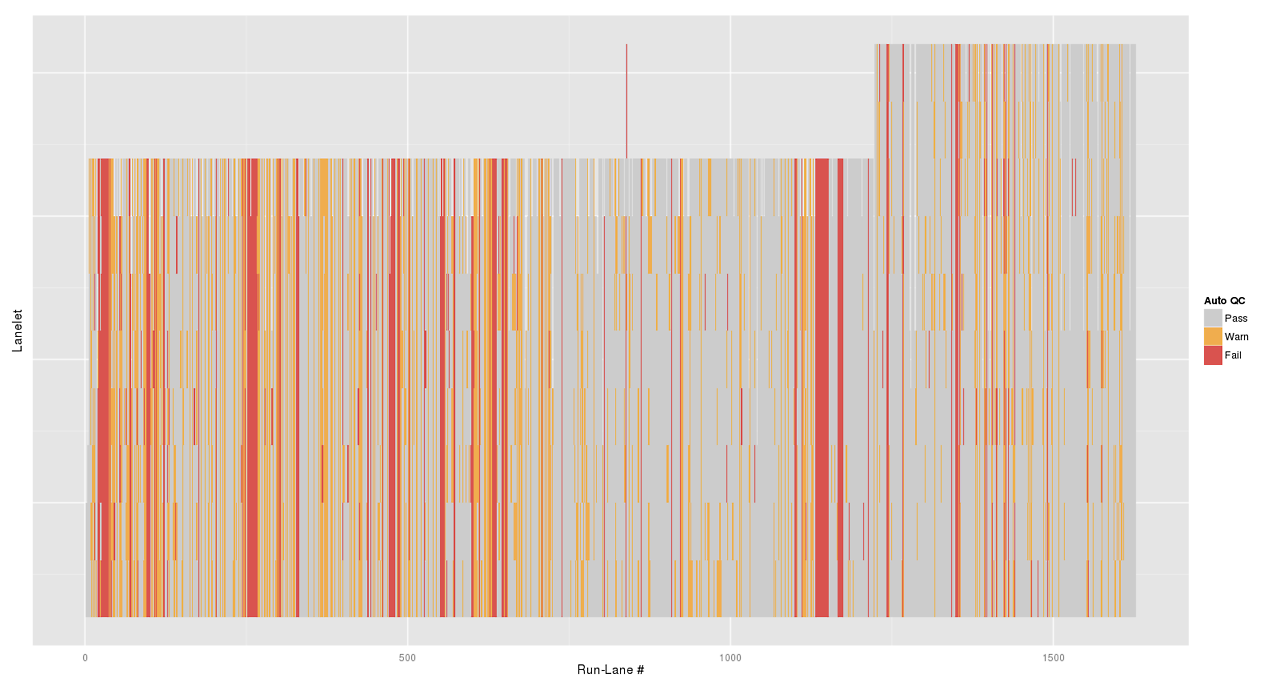
\includegraphics[width=1.0\textwidth]{classcorr}
    \caption[ClassCorr]{\textbf{Heatmap of lanelet QC status by lane}: Lanes are
    vertical bars with each lanelet cell coloured red to represent a failure,
yellow for a warning and grey for a pass.}
    \label{fig:classcorr}
\end{figure}

%TODO affected effected?
In such a case there would appear to exist a relationship between the respective
qualities of each lanelet in a lane as well as each lane in a sequencing run. To
examine this further, an R script utilising \textbf{ggplot2} was authored to
visually inspect whether correlation existed and if so to what degree that data
is affected.

Figure~\ref{fig:classcorr} displays a plot of \textbf{auto\_qc} classification
for each lanelet in a lane. The plot itself is a dense heatmap
where each lane stands as a vertical bar, broken in to horizontal cells, each
of which represents a lanelet that was sequenced in that particular lane. These
lanelets are colour coded using; red for failures, yellow for warnings and grey
for passes (to allow the other two classes to be more easily seen).

Therefore an unbroken vertical red line indicates that all lanelets that
comprise of that line failed to pass some aspect of the current
\textbf{auto\_qc} thresholds. In reality there are few conditions under which
a lanelet would fail irrespective of the status of the rest of the lanelets in
the same lane which typically involve an error during the preparation of the
sample (an easy to spot result as it will cause poor quality across all lanelets
using that sample).

%TODO Better explanation
Overall there are a series of instances appearing to support correlation for
whole-lane failures and warnings but despite this there do appear to be occasions
where a lanelet has failed where the remainder of the lane has not.
Having discussed this with the project supervisor and contacts at the Sanger Institute we decided to continue to
the implementation stage, agreeing that whilst some evidence of correlation
between lanelets in the same lane has emerged, we will still be able to recover
parameters that will be useful to quality control and statistical testing may be
required following this analysis to describe how powerful such parameters are
taking this possible correlation in to account.

It should be
noted that the proportion of failures and warnings is considerably smaller than
passes and so care will need to be taken to find a balance; for example it would
not be feasible to merely discard lanelets from lanes that have failed entirely
as there'd hardly be any data on which to train a classifier. Indeed other
solutions may be possible, perhaps weighting observations which exhibit similar
behaviour to other lanelets in their lane so as to give their parameter values
less priority during the construction of the classifier itself.

It is worth noting that although the plot does not make a particular
distinction between lanes in the same flow cell, lanes are sequentially
identified so the red bars of thicker-width arguably display some failures
across entire flow cells.

As a final note it should be stressed that this plot should be regarded as a
diagnostic rather than an experiment with a direct conclusion. Given more time it
would be useful to investigate the nature of these possible correlations, given
a lane that has failed across all lanelets: do those lanelets actually express
similar quality metrics?

%%%%%%%%%%%%%%%%%%%%%%%%%%%%%%%%%%%%%%%%%%%%%%%%%%%%%%%%%%%%%%%%%%%%%%%%%%%%%%%
\section{Recovering Ratios}

An initial scan of the summary numbers available in the "bamcheckr'd" files
introduced in Chapter~\ref{chap:bamcheckr-data} revealed 82 different
parameters. However, when comparing this parameter set to the threshold rules of
\textbf{auto\_qc}, it appeared that some parameters were "missing".

In the pursuit of replicating the decisions of the
existing system, it is ideal to have all the parameters used in the making of
those decisions at hand. In particular, the missing parameters were of a
normalised nature, typically in the form of a ratio or percentage which should
make them more valuable than a parameter that just represents a raw count of
some property.

It was found that these missing parameters are calculated in a step preceeding
\textbf{auto\_qc} as part of the \textbf{vr-pipe}
pipeline\footnote{https://github.com/wtsi-hgi/vr-pipe/blob/hgi-release/modules/VRPipe/Steps/vrtrack\_auto\_qc\_hgi\_3.pm}.

%...It is actually here that the hard-coded thresholds for warnings and failures
% are applied and the target decision is made too!

Whilst I could have attempted to set-up my own instance of \textbf{vr-pipe} to
recover this data, speaking with contacts at the Sanger Institute, it was
decided that this would prove troublesome work; requiring an involved
deployment to a cloud based facility such as Amazon's Elastic Compute Cloud and
installation of various Perl dependencies as well as requiring access to many
controlled databases within the institute.

Most of the functions that calculated these parameters turned out to be
straightforward and could easily be ported to another application. At first
it was intended to add these functions to the program authored for this part of
the project, but the Sanger Institute suggested it would be more useful to
implement such functionality in \textbf{bamcheckr} directly, removing some of
\textbf{auto\_qc}'s dependence on its position in \textbf{vr-pipe}.

\begin{listing}[H]
    \caption[r-dev]{: Installing an in-development R package with \textbf{devtools}}
    \label{list:r-dev}
    \begin{minted}[mathescape,
                %linenos,
                numbersep=5pt,
                gobble=8,
                frame=lines,
                framesep=2mm]{r}
        # Install and include the `devtools' package
        install.packages("devtools")
        library(devtools)

        # Install package directly from Github repository
        install_github("samstudio8/seq_autoqc", subdir="bamcheckr")

        # Install package from local directory
        install("/home/sam/Projects/seq_autoqc/bamcheckr")

    \end{minted}
\end{listing}

With the help of \textbf{devtools}\citep{man:devtools} (see
Listing~\ref{list:r-dev}) it was simple to develop and test contributions to
\textbf{bamcheckr} locally without needing to re-publish the package after
changes. An additional script was added to \textbf{bamcheckr}'s NAMESPACE... to
recover the missing ratio and percentage based parameters...

...unfortunately, the performance of the script was poor, taking 5.5s on average
and increasing to 16.1s when enabling a complex function containing many vector
operations (potentially inefficient due to my lack of R experience)...
for overlapping\_base\_duplicate\_percentage

...utilising the program designed and implemented in the following chapter...
loaded required information and used the API to calculate the missing
parameters...

...Morandat\citep{morandat-rperf}

%FUTURE
...with such an intriguing difference in performance with significantly more
time it would be appealing to explore the idiosyncrasies of each implementation
...although such an investigation would quite likely sufficiently generate an
entire project of its own.



%%%%%%%%%%%%%%%%%%%%%%%%%%%%%%%%%%%%%%%%%%%%%%%%%%%%%%%%%%%%%%%%%%%%%%%%%%%%%%%
\section{Contributions to bamcheckr}
...R CMD BATCH issue
...Fixed a graph plotting failure.


\chapter{Frontier}
\ifpdf
    \graphicspath{{Chapter3/Figs/Raster/}{Chapter3/Figs/PDF/}{Chapter3/Figs/}}
\else
    \graphicspath{{Chapter3/Figs/Vector/}{Chapter3/Figs/}}
\fi

%%%%%%%%%%%%%%%%%%%%%%%%%%%%%%%%%%%%%%%%%%%%%%%%%%%%%%%%%%%%%%%%%%%%%%%%%%%%%%%

This chapter introduces \textbf{Frontier}: the main programming effort for this
part of the project. \textbf{Frontier} is a Python package that serves as a data manager,
providing both interfaces to read inputs into structures in memory and to
retrieve them in formats acceptable to a machine learning framework.

Appendix~\ref{app:pre-frontier} describes some analysis performed before
implementation of \textbf{Frontier}.

\section{Design}
\subsection{Purpose}

\textbf{Frontier}'s purpose is to supplement analysis with \textbf{scikit-learn} by
allowing a user to read in and parameterise data in a format that can then be
used for analysis by the \textbf{scikit-learn} library.  \textbf{Frontier} is designed
to simplify the process of setting up machine learning tasks and enable
experiment repeatability by removing the need for users to spend time
constructing classes and functions to parse their input data and to just get on
with analysis using \textbf{scikit-learn}.

Initially \textbf{Frontier} was to act as a wrapper around \textbf{scikit-learn},
essentially removing the end user's interaction with the library and merely
providing an interface for data to be passed in and some sort of classifier to
be returned. However this quite clearly limited \textbf{Frontier}'s audience by tying it
to a particular framework and would quickly become unmanageable in the task of
providing wrappers for all aspects of an external library.

Instead is far better to allow \textbf{Frontier} to be used alongside a user's chosen
machine learning framework, providing a useful API to parse and extract
observations and variables from input data and arrange them in structures
suitable for processing with \textbf{scikit-learn}.

If possible, \textbf{Frontier} could also handle any objects returned, displaying or
logging any textual or graphical information pertaining to a returned
classifier's accuracy to assist a user in the ongoing performance monitoring of
changes to used data subsets or parameters.


\subsection{Format}

\textbf{Frontier} is designed as a Python package, allowing a user to import its
functionality into other programs. The result of this project's technical
output could almost be considered as two separate entities: \textbf{Frontier} itself, the
package designed to ease user interaction with scikit-learn and \textbf{Front},
a Python script which implements \textbf{Frontier}'s functionality in order to interact
with scikit-learn to conduct analysis on the \textbf{auto\_qc} data.


\subsection{Method}
\label{sec:frontier-method}

\textbf{Frontier} is the result of abstracting code and tools created during
the use of \textbf{scikit-learn} for analysis of the current \textbf{auto\_qc}
system. Whilst scripts initially hard-coded to suit the specific needs of the
project -- with hard coded classes and encodings -- \textbf{Frontier} followed
an evolutionary design process and grew to become a more generic framework
applicable to learning tasks outside of this study.


%%%%%%%%%%%%%%%%%%%%%%%%%%%%%%%%%%%%%%%%%%%%%%%%%%%%%%%%%%%%%%%%%%%%%%%%%%%%%%%
\section{Concepts}

Appendix~\ref{app:concepts-p1} introduces some ideas that will assist
understanding of the application's purpose and terminology used in the following
implementation section.

%%%%%%%%%%%%%%%%%%%%%%%%%%%%%%%%%%%%%%%%%%%%%%%%%%%%%%%%%%%%%%%%%%%%%%%%%%%%%%%
\pagebreak
\section{Implementation}

This section investigates the implementation of \textbf{Frontier}'s major components:

\begin{itemize}
    \item Informing the package of the problem domain...
    \item Interfaces provided for reading in data
    \item Storage of read data in memory
    \item Retrieval of stored data for interaction with \textbf{scikit-learn}
\end{itemize}


\subsection{Class Definitions}
\label{chap:classes}

\textbf{Frontier} is designed to support classification machine learning problems, to
adequately support this task, the package must be aware of each of the possible
classes in the problem space. Early versions of \textbf{Frontier} were specifically
designed for training and testing data from \textbf{auto\_qc} and could only
support encoding and decoding of the pass, fail and warn classes.

However this implementation was clearly esoteric and held little to no further
use outside the domain of the project's learning task. What would happen if a
class label were to be added or removed in future? Most likely many lines of
code would need to be re-written to handle such cases; the package was
inflexible.

To counter this, \textbf{Frontier} was refactored to remove hard coded label definitions
enabling its use as a more general purpose tool where users can specify the
domain's classes and their associated labels and encodings.
Listing~\ref{list:FrontierClasses} shows the definitions used by Front to work
with the \textbf{auto\_qc} data.

\begin{listing}[H]
    \caption[FrontierClasses]{: Class definitions for \textbf{auto\_qc} as passed to \textbf{Frontier}}
    \label{list:FrontierClasses}
    \begin{minted}[mathescape,
                %linenos,
                numbersep=5pt,
                gobble=8,
                frame=lines,
                framesep=2mm]{python}
        CLASSES = {
                "pass": {
                    "names": ["pass", "passed"],
                    "code": 1,
                },
                "fail": {
                    "names": ["fail", "failed"],
                    "code": -1,
                },
                "warn": {
                    "names": ["warn", "warning"],
                    "code": 0,
                },
        }
    \end{minted}
\end{listing}

As per Listing~\ref{list:FrontierClasses}, to define classes a user must provide
a Python dict containing the following for each label:

\begin{itemize}
    \item \textbf{class} \textit{String}\hfill\\
        The dictionary key is used as the canonical name of the class label
    \item \textbf{names} \textit{[String]}\hfill\\
        A list of labels that denote membership of this class
    \item \textbf{code} \textit{Integer}\hfill\\
        The encoded representation of this class (See Chapter~\ref{chap:labelcode})
    \item \textbf{\_recode} \textit{Boolean, Private}\hfill\\
        A flag to indicate whether an API action has changed the code of this
        class, typically used when treating all members of one class as a member
        of another -- A user should never set this manually
    \item \textbf{\_count} \textit{Integer, Private}\hfill\\
        The number of observations with this label, typically used when
        calculating weightings based on the proportions of class sizes and
        outputting logging information -- A user should not set this manually
\end{itemize}

This simple structure allows \textbf{Frontier} to be compatible with almost any
classification learning task with minimum input from the end user. Additional
utilities provided by the \textbf{Frontier} utils subpackage use this structure to
automatically classify and encode labels without user intervention with the
following functions:

\begin{itemize}
    \item \textbf{classify\_label} \hfill\\
        Attempt to classify a label by comparing a given string to each set of
        \textit{names}, locating an exact match will return the relevant
        canonical class label
    \item \textbf{encode\_class} \hfill\\
        Given a canonical class label, return its \textit{code}
    \item \textbf{decode\_class} \hfill\\
        Given a \textit{code}, return the canonical class label unless
        \textit{\_recode} is True
    \item \textbf{count\_class} \hfill\\
        Increment the \textit{\_count} for a particular class given its
        canonical label
\end{itemize}

These functions are put to use throughout \textbf{Frontier} and are essential for reader
classes (detailed in the next chapter) to parse, classify and then encode
observation targets automatically from relevant files.


\subsection{Input Handling}
\label{sec:frontier-input}

\textbf{Frontier}'s modular nature allows users to write their own Python classes to read
data from any form of input file or stream. Two examples of which are the
classes used to read from the "bamcheckr'd files" documented in
Appendix~\ref{app:bamcheckr} and the \textbf{auto\_qc} decisions matrix briefly
demonstrated in Appendix~\ref{app:aqc_matrix}.

These classes are described as \textbf{Readers} and implement a common base
class, \textbf{AbstractReader} which takes care of
setting up the file handler, including functions to both close and iterate over
the file's contents. It will also automatically call its own
\textbf{process\_file} function that skips over any header lines before passing
each line in the file stripped of any newline characters to \textbf{process\_line}.

It is expected that derived classes will at least provide their own
implementations for \textbf{process\_line} and \textbf{get\_data}. Failing to do
so will cause \textbf{Frontier} to throw a \textbf{NotImplementedError} when attempting
to use the class to read data.

\textbf{process\_line} defines the line handling operations that extract and store
desired data found in a given line. This responsibility includes returning None
for lines that contain comments and irrelevant data and conducting any necessary
sanitisation (the \textbf{BamcheckReader} for example makes use of a utility
function to translate spaces, underscores and dots to hyphens).

\textbf{get\_data} must return any read in data in a suitable structure for
storage by \textbf{Frontier}. Typically this will be a Python dictionary using some
unique identifier for each observation as a key, mapping to an arbitrary value
or object containing that observation's parameters. Further discussion on
\textbf{Frontier}'s storage of data and targets is to follow.

The \textbf{AbstractReader} class is designed to simplify the process of reading
in observations and their targets for end users, however it is still up to the
author of the derived class to set up any structures to store data (which cannot
be done automatically without likely enforcing potentially unhelpful
constraints) before initialisation of the inherited base class (via the call to
\textbf{super}) as shown in Listing~\ref{list:superreader}.

\begin{listing}[H]
    \caption[superreader]{: Extract from \textbf{BamcheckReader} class
        documenting initialisation of necessary data structures and calling
        for initialisation of its inherited base class}
    \label{list:superreader}
    \begin{minted}[mathescape,
                %linenos,
                numbersep=5pt,
                gobble=8,
                frame=lines,
                framesep=2mm]{python}
        class BamcheckReader(AbstractReader):
            [...]

            def __init__(self, filepath, CLASSES, auto_close=True):
                self.summary = SummaryNumbers()
                self.indel = IndelDistribution()
                super(BamcheckReader, self).__init__(filepath, CLASSES, auto_close, 0)

            [...]
    \end{minted}
\end{listing}

As shown in Listing~\ref{list:superreader}, the initialisation of the
\textbf{AbstractReader} allows four arguments:

\begin{itemize}
    \item \textbf{filepath} \textit{String}\hfill\\
        A relative or absolute path to a file from which to extract data or
        targets
    \item \textbf{CLASSES} \textit{Dictionary}\hfill\\
        A dictionary of user specified class labels defined as described in
        the previous chapter
    \item \textbf{auto\_close} \textit{Boolean, Optional}\hfill\\
        Whether or not to close the file handle immediately after executing
        \textbf{process\_file}, this is True by default to prevent either memory
        leaking when users are reading in a large number of files and are
        perhaps unaware that they require closing or the throwing of an IOError
        caused by having too many file handles open at once
    \item \textbf{header} \textit{Integer, Optional}\hfill\\
        The number of lines to ignore before the reader should begin
        passing stripped lines to \textbf{process\_line}, defaults to 0
\end{itemize}

Currently it is also the responsibility of the author of a derived class to
perform relevant sanity checking of any extracted data. For example the
\textbf{BamcheckReader} class checks for the presence of multiple entries of a
particular metric which will print a notice if found, unless the entries have
differing values, upon which an exception is thrown and the process is halted.

Once a reader has been defined for a particular file format, a user need only
provide a directory of files to be parsed and the name of the class designed to
complete the parsing. \textbf{Frontier} will then take care of executing the parsing
process on all files in the directory. After a derived reader has completed file
handling, \textbf{Frontier} will call its \textbf{get\_data} function to
"move"\footnote{Rather, a pointer to the address of the extracted data's
dictionary hashmap will be copied to memory inside a \textbf{Frontier} class} the
extracted data to its own storage.

At this point \textbf{Frontier} will also check the integrity of the data, primarily
that all parameters have a non-zero variance\footnote{Using an algorithm for
accurately computing running variance introduced in Donald Knuth's \textit{Art
of Computer Programming}\citep{knuth1998art-variance}}. Users will be warned
when this requirement is violated; parameters with no variance cannot provide
much information for successful classification as their values are equal for
all class labels!

%FUTURE
In future it would be useful to investigate whether it would be feasible to
perform such sanity checking in a generic manner to ensure it could be applied
to a wide enough range of scenarios to make it worth including functionality in
the \textbf{AbstractReader} directly.

With more time, future improvements could overhaul the reader interfaces
to allow users to simply specify the format of a file in a string that can be
parsed by \textbf{Frontier}'s IO subpackage, rather than having to write their own derived
class. Classes could also list file extensions they are capable of processing
which could potentially be used to automatically determine which readers to use
without requiring the user to explicitly specify.


\subsection{Storage}

\textbf{Frontier} specifies a class called the \textbf{Statplexer}\footnote{A somewhat
contrived contraction of 'Statistics Multiplexer'} which provides users with a
single point of access to all read in data. The reader interfaces described in
the previous chapter implement their own loading functions to populate the
\textbf{\_data} and \textbf{\_targets} class members of the \textbf{Statplexer}
object, both of which are Python dictionaries.

During the parsing of observation data with the relevant reader class, the
reader is expected to locate an appropriate unique ID for each observation. In
the case of processing of \textbf{auto\_qc} data, this would be the lanelet's
barcode which is collected from the filename of that particular lanelet's
"bamcheckr'd" file.
This identifier is then used as a key in both the \textbf{\_data} and
\textbf{\_targets} dictionaries to map to a structure (typically another
dictionary or an arbitrary class) that stores that observation's parameters
and its known target (encoded class label), respectively.

Although these attributes can be manipulated directly (and indeed they are for
testing purposes) the leading underscore follows a popular convention defined in
Python's style guideline, PEP8\citep{pep8}, where class members with leading
underscores should be treated as non-public. Python doesn't have private
variables such as those that may be found in other languages like Java, indeed
the Python style guide points out that "no attribute is really private in
Python"\citep{pep8}. In an interesting StackOverflow answer on the subject, a
user describes that this is "cultural"\citep{so:pythonprivate} and that Python
programmers are trusted not to circumvent convention and "mess around with those
private members". Users are therefore expected to use the functionality
\textbf{Frontier} provides for controlled getting and setting of data stored in these
pseudo-private \textbf{\_data} and \textbf{\_targets} members.

\textbf{load\_data}, for example, should be used exclusively when populating
the two dictionaries and is automatically called on construction of the
\textbf{Statplexer} if the construction arguments are valid.
\textbf{load\_data} will automatically call other necessary (pseudo-private)
functions of the class including \textbf{\_test\_variance} which checks that
parameter variances are non-zero and also warns users if new observations
are overwriting old ones, or if an observation does not appear to have a
corresponding target.

The following section details the retrieval of data and targets from the
\textbf{Statplexer} which are returned to the user in \textbf{NumPy} arrays. Why
does \textbf{Frontier} not just store the read in data in such a structure to
begin with?

This is primarily due to the underlying layout of a list structure as introduced
in Appendix~\ref{sec:python-structures}. Given the nature of input data,
the number of observations and parameters are unknown before the input
data is actually read and so memory cannot be reserved to prevent these operations.
The potential number of input files renders reading through the data once to
reserve the right amount of memory for a second read-through impractical in
terms of time.

It is arguable that despite this, the data could be unloaded from the
\textbf{\_data} and \textbf{\_targets} dictionaries into some form of array at
the end of the call to \textbf{load\_data}. However as the \textbf{Statplexer}
allows loading of additional data at any time, which would not only risk
increasingly expensive resizing operations as the list continues to expand but
the sanity checking that takes place in \textbf{load\_data} involves checking
for membership of a given ID in \textbf{\_data} and \textbf{\_targets} which is
constant for dictionaries and significantly slower for large lists (see
Appendix~\ref{sec:python-structures}).

It is possible that an implementation could use both a dictionary and an array;
appending the observations to the array and entering a mapping between the
observation ID and its index in the array.  Though this would still not avoid
the issue of relocating the array once it grows beyond its bound in memory.

Worse still, as results requested from the \textbf{Statplexer} API are returned
to the user in a sorted matrix\footnote{A two-dimensional \textbf{NumPy} array}
(\textit{i.e.} rows and columns are ordered alphanumerically by the observation
ID and parameter name, respectively), if observations are not processed in a
sorted order (which is not a requirement) then returning results will involve
accessing the proposed \textbf{\_data} and \textbf{\_targets} arrays in a
non-linear fashion, losing any efficiency that could be gained from using an
array in the first place.

Whilst not entirely optimal\footnote{Dictionaries still require use of
\textbf{sorted} when creating a result matrix via the API}, in terms of a
compromise between memory complexity and avoiding expensive operations on data
input and retrieval, dictionaries offer the best balance.

It should be noted that the \textbf{Statplexer} stores a copy of the user
defined CLASSES dictionary (as the class member \textbf{\_classes}), which is an
argument to its construction, allowing the \textbf{Statplexer} to share this
information with any readers or utility functions who require it.


\subsection{Retrieval}

\textbf{Frontier}'s \textbf{Statplexer} is designed to provide functions to an
end user for extracting desired data in a format suitable for passing as an
argument to functions of an external framework or library, such as
\textbf{scikit-learn}. As specified in \textbf{Frontier}'s purpose, the package
must provide user-friendly functions to extract observations and parameters of
interest from the internal \textbf{Statplexer} representation.

The previous section suggests that directly accessing elements of the
\textbf{Statplexer}'s \textbf{\_data} and \textbf{\_targets} member dictionaries,
whilst possible, would violate the psuedo-private nature of the variables and even
so, this would hardly be a user friendly way in which to obtain data from the
\textbf{Statplexer}.

As described in Section~\ref{sec:frontier-method}, development of
\textbf{Frontier} was evolutionary, growing to meet the needs and requirements
of the underlying machine learning problem that this project strives to solve.
It became clear that in trying many combinations of observation and parameter
subsets that \textbf{Frontier} would need to provide not just a function to
return the contents of \textbf{\_data} and \textbf{\_targets} but to assist in
retrieving similar subsets automatically with as little effort from the end user
as possible.

But how can a user make an informed decision on parameters to subset?
Though this is primarily the role of feature selection, which will be discussed
later in this chapter, firstly a user will need to have a feeling for what
parameters are actually present and ideally be offered functionality to
allow for quick elementary exploration of that set. For this, \textbf{Frontier}
can be used to inspect the parameters extracted from the observations via the
functions:

\begin{itemize}
    \item \textbf{list\_parameters} \hfill\\
        Return a sorted list of all parameters
    \item \textbf{find\_parameters} \hfill\\
        Given a list of input strings, return a list of parameters which contain
        any of those strings as a substring
    \item \textbf{exclude\_parameters} \hfill\\
        Given a list of input strings, return a list of parameters which do not
        contain any of the input strings as a substring, or if needed an exact
        match
\end{itemize}

Once users have an idea of the parameters they wish to extract from each
observation, \textbf{Frontier} maintains an additional set of functions that act
as a form of API, allowing users to retrieve subsets of data based on both
parameters and targets:

\begin{itemize}
    \item \textbf{get\_data\_by\_parameters} \hfill\\
        Return data for each observation, but only include columns
        for each parameter in the given list
    \item \textbf{get\_data\_by\_target} \hfill\\
        Return data for each observation that have been classified in one of the
        targets specified and additionally only return columns for the
        parameters in the given list
\end{itemize}

%TODO Figure to show mapping between container elements
The prior section first introduces the format in which data is returned, the
two-dimensional \textbf{NumPy} array -- referred to as the \textit{Frontier Results
Matrix} -- in which a row represents a particular observation and each column
represents a parameter (or feature). By default both dimensions are
ordered alphanumerically; rows are sorted by their observation ID, columns by
the parameter name\footnote{Typically the 'cleaned' or otherwise sanitised
    parameter name, as noted in Section~\ref{sec:frontier-input} for example
where the \textbf{BamcheckReader} class will automatically convert spaces and
other predefined characters to hyphens.}. Targets are also returned in a
\textbf{NumPy} array, with each index of the target array mapping 1:1 with the
observation row of the same index in the \textit{Results Matrix}.


\subsection{Logging}

Section~\ref{sec:part1:testing} concluded that time constraints would not allow
significant effort to be invested in building a platform for cataloguing results
from test runs of the classifier. I decided to settle for populating fields in a
structured text file, an example of which can be found in
Appendix~\ref{app:frontier-log}.

\textbf{Frontier} provides functions such as \textbf{write\_log} to dump
\textbf{Statplexer} parameters to a given file path along with cross-validation
performance associated with a particular training and prediction run of a
decision tree classifier. Such files can easily be manipulated with common
command line tools such as \textbf{grep} and the text processing language,
\textbf{awk}.

Given the time to create specialised software for storing and comparing
different runs of the classifier in future, it would be trivial to import old
\textbf{Frontier} log files.


\section{Usage Example}

\begin{listing}[H]
    \caption[callstatplexer]{\textbf{Constructing a Statplexer}: Syntax for
    instantiation of \textbf{Frontier}'s \textbf{Statplexer}.}
    \label{list:callstatplexer}
    \begin{minted}[mathescape,
                %linenos,
                numbersep=5pt,
                gobble=8,
                frame=lines,
                framesep=2mm]{python}

        from Frontier import frontier
        from Frontier.IO import DataReader, TargetReader

        data_dir = "/home/sam/Projects/owl_classifier/data/"
        target_path = "/home/sam/Projects/owl_classifier/targets.txt"

        CLASSES = {
                "hoot": {
                    "names": ["owl", "owls"],
                    "code": 1,
                },
                "unhoot": {
                    "names": ["cat", "dog", "pancake"],
                    "code": 0,
                },
        }

        statplexer = frontier.Statplexer(data_dir,
                                         target_path,
                                         CLASSES,
                                         DataReader,
                                         TargetReader)
    \end{minted}
\end{listing}

Constructing the Statplexer requires the following arguments:

\begin{itemize}
    \item \textbf{data\_dir} \textit{String}\hfill\\
        Root data directory under which all files will be parsed for observation data
    \item \textbf{target\_path} \textit{String}\hfill\\
        Path to file to be parsed for observation targets
    \item \textbf{CLASSES} \textit{Dictionary}\hfill\\
        A dictionary of user specified class labels defined as described in
        Chapter~\ref{chap:classes}
    \item \textbf{DataReader} \textit{Module}\hfill\\
        Module containing the class (of the same name) to be used to parse each
        file in the \textit{data\_dir} tree for observation data
    \item \textbf{TargetReader} \textit{Module}\hfill\\
        Module containing the class (of the same name) to be used to parse the
        \textit{target\_path} file for target data
\end{itemize}

%TODO Add to example
\begin{listing}[H]
    \caption[callstatplexer]{\textbf{Retrieving Data}: Example usage of
    \textbf{Frontier}'s \textbf{Statplexer} API.}
    \label{list:callstatplexer}
    \begin{minted}[mathescape,
                %linenos,
                numbersep=5pt,
                gobble=8,
                frame=lines,
                framesep=2mm]{python}
        statplexer.find_regressors(["mean", "percent", "rate", "average"])
    \end{minted}
\end{listing}


\section{Testing}

\textbf{Frontier} is bundled with a small testing suite designed to flex the
functionality of the two included readers (\textbf{AQCReader} and
\textbf{BamcheckReader}) as well as both the \textbf{Frontier} utilities and
the \textbf{Frontier} API itself. The suite consists of three Python scripts
which utilise the \textbf{unittest}\citep{py-unittest} package in the Python
standard library.  The scripts are located in the \textit{tests} directory of
the \textbf{Frontier} package.

\subsection{AQCReader and BamcheckReader}

Both of \textbf{Frontier}'s included readers are distributed with their own
modest test suite, designed to test the particular functionality of that reader,
including; cleaning or sanitisation of data, ensuring warnings or exceptions are
thrown when duplicate observations are encountered as required and that the two
readers are capable of returning data and labels that were expected for a given
observation.

\subsection{Frontier Utilities}

Members of the utilities package responsible for
encoding and decoding of class labels and class codes are checked to ensure that
they return the expected values. The suite also checks whether relevant exceptions
are raised when unknown class labels or codes are encountered.

\subsection{Frontier API}

Testing \textbf{Frontier} itself is significantly more complicated, to
accomplish the feat, a test data set with various observations, parameters and
targets is automatically generated by the testing suite.  The suite then
examines the results of the various API calls to ensure that each returned set
of data and targets, include or exclude observations as expected.  Tests also
ensure that the API behaves appropriately for incorrect user input, including
incorrect or completely unknown parameters and targets.


%%%%%%%%%%%%%%%%%%%%%%%%%%%%%%%%%%%%%%%%%%%%%%%%%%%%%%%%%%%%%%%%%%%%%%%%%%%%%%%
\chapter{Results}

This chapter examines the main results from application of \textbf{Frontier} and
\textbf{scikit-learn} to our \textbf{auto\_qc} learning task.

\section{Introduction}

To recap...

\begin{itemize}
    \item Set up environment for decision tree classification...
    \item Select an appropriate set of parameters to use...
    \item Minimise decision tree...
    \item Apply best practice..
    \item Best parameters...?
    \item Identified any parameters that match or not?
\end{itemize}

\section{Introduction}
\subsection{Why Decision Trees?}
%TODO Citations...

...each node represents a test on the value of an attribute or feature

...single discrete target
...primarily human readable rule set... like a flow chart...
...simple to interpret, can be statistically verified
...robust to noise
...realistic applications in medicine and risk
...algorithm capable of scaling to relatively large sets such as ours
...at this time we're not looking for a "black box"
...want to be able to see whether the current rule set can be extracted with
machine learning methods...

...decisions tree however are prone to overfitting -- failing to generalise...
...cannot promise optimality
...duplicated subtrees
...cannot be applied to first order logic, only one parameter can be tested at a
time, future tests are not "aware" of previous tests

\subsection{DecisionTreeClassifier}
% TODO Cite
% http://scikit-learn.org/stable/modules/generated/sklearn.tree.DecisionTreeClassifier.html
...gini impruty or information gain... scikit seems to favour gini...
...

\begin{itemize}
    \item \textbf{max\_depth} \hfill\\
        ...
    \item \textbf{min\_samples\_split} \hfill\\
        ...
    \item \textbf{min\_samples\_leaf} \hfill\\
        ...
    \item \textbf{min\_features} \hfill\\
        ...
\end{itemize}

...Classification And Regression Tree (CART)





\section{Parameter Sets and Selection}
\subsection{Naive Parameter Sets}

Identified a series of parameter sets for initial training and testing purposes:

\begin{itemize}
    \item \textbf{AQC} \hfill\\
        A set consisting of all available parameters used by \textbf{auto\_qc}.
    \item \textbf{AQCN} \hfill\\
        Replaces groups of the \textbf{AQC} set with aggregated parameters.
    \item \textbf{ERROR} \hfill\\
        An experimental toy set consisting of only the "error-rate" parameter.
    \item \textbf{NO\_ERROR} \hfill\\
        Another toy set designed to test results gained by excluding the
        "error-rate" parameter.
    \item \textbf{BASELINE} \hfill\\
        Include any parameter which include "baseline" as a substring.
    \item \textbf{NOBASELINE} \hfill\\
        Exclude any parameter which include "baseline" as a substring.
    \item \textbf{MARP} \hfill\\
        Include any parameter which includes one of the following substrings:
        mean, percent, rate or average.
    \item \textbf{NO\_MARP} \hfill\\
        Exclude any parameter which includes one of the following substrings:
        mean, percent, rate or average.
\end{itemize}

Of note in particular is the \textbf{AQC} set, constructed from the parameters
available from the "BAMcheckr'd" data that are taken in to account by the
current \textbf{auto\_qc} system. It should be noted however that not all these
parameters were initially available in the input files and \textbf{auto\_qc}
relies upon data made available from \textbf{vr-pipe} where the rules of
\textbf{auto\_qc} are actually applied. Appendix~\ref{app:ratios} discusses
contributions I made to \textbf{bamcheckr} for recovering these parameters for
use in our analysis. Ultimately, \textbf{bamcheckr} performed too slowly and it
was possible to use \textbf{Frontier} itself to extract the additional features
needed to better represent the decisions made by the current system.

%TODO Cite dtc
For each parameter set, data and targets were extracted via \textbf{Frontier}'s
API before being subset by \textbf{scikit-learn}'s \textbf{StratifiedKFold}
function. All available data (13,455 "BAMcheckr'd" lanelets) were used as input,
the target variable could be one of three classes; pass, fail or warn.
The subsets are referred to as "folds" (of which we used 10) and for
each fold a \textbf{DecisionTreeClassifier} was trained and tested.
Table~\ref{tab:pset-cv} outlines the average cross validation scores across each
such experiment.

\begin{table}[H]
    \centering
    \begin{tabular}{l | c  c  c  c  r}
        Set           & Nº & CV ± SD & SCV ± SD & Depth & Most Important Feature\\
        \hline
        ALL           & 86 & 90 ± 4 & 97 ± 1 & 38 & T-percent-max-baseline-deviation (27\%)\\
        AQC           & 27 & 87 ± 4 & 95 ± 1 & 36 & T-percent-max-baseline-deviation (31\%)\\
        AQCN          & 21 & 86 ± 4 & 95 ± 1 & 39 & max-max-baseline-deviation (31\%)\\
        ERROR         & 1  & 60 ± 6 & 61 ± 2 & 53 & error-rate (100\%)\\
        NO\_ERROR     & 85 & 90 ± 4 & 97 ± 1 & 38 & T-percent-max-above-baseline(27\%)\\
        BASELINE      & 34 & 82 ± 5 & 89 ± 1 & 46 & T-percent-max-above-baseline(28\%)\\
        NOBASELINE    & 52 & 72 ± 10 & 91 ± 1 & 31 & error-rate (24\%)\\
        MARP          & 47 & 87 ± 4 & 95 ± 1 & 39 & T-percent-max-above-baseline (27\%)\\
        NO\_MARP      & 39 & 75 ± 7 & 87 ± 1 & 38 & max-max-baseline-deviation (34\%)\\
    \end{tabular}

    \caption[pset-cv]{\textbf{Parameter Set Cross Validation Scores}: Results of
        classifying testing data in to one of three classes; pass, fail or warn.
        Columns left to right; parameter set name, number of parameters
        included, average cross-validation score (max 100) ± std. deviation,
        average stratified cross-validation score (max 100) ± std. deviation,
        average depth of the generated tree and the most important parameter by
        Gini importance (max 100). Tree depth and parameter importance was
    estimated on experiments using the stratified data.}

    \label{tab:pset-cv}
\end{table}

Whilst these parameter sets are certainly crude -- a majority of them having
been constructed without close examination just by matching or excluding
substrings using \textbf{Frontier}'s parameter inspection functions -- we can
learn quite a lot about the available data.

Firstly it should be of no surprise that the \textbf{ALL} model scores highly in
both cross-validation and stratified cross-validation testing. The feature group
is a superset over the same parameters used by \textbf{auto\_qc} itself.
Similarly the \textbf{NO\_ERROR} set which uses all but one parameter
(\textbf{error-rate}) scores highly.

It's interesting to compare the scores between the \textbf{AQC} and
\textbf{AQCN} parameter sets against \textbf{ALL}. Both of the former score
highly despite having significantly fewer parameters. This appears to indicate
that many of the parameters in the \textbf{ALL} model are redundant for use in
classification. This should of course be expected, you'd hope to see that a set
that includes parameters known to be used by the current \textbf{auto\_qc} system
is capable of replicating results made by that system.

In general the other models perform reasonably well, potentially reflecting the
simple linear nature of the decisions made by the \textbf{auto\_qc} system.

Stratified cross-validation scores are consistently better and less variable
(smaller standard deviations) than their non-stratified counterparts. This
should be due to the more "balanced" training and testing sets
gained by assigning observations to folds to match their proportions in the
whole data set. The differences between the pairs of validation scores is
predictable -- averaging 8.66 percentage points -- but the \textbf{NOBASELINE}
set presents a difference of almost 20pp and exhibits more variable behaviour.
This suggests that excluding the baseline related parameters is problematic for
one (or two) of the three class labels (as the only difference expected between the
experiments will be the proportions of the classes).


...highlights the shortcomings of using a decision tree...
overfitting... gini coefficient not a real measure of importance...

\subsection{Informed Parameter Selection}

Whilst the crude parameter sets of the previous section were useful to gain
understanding of the data that we have, it was necessary to obtain more
deliberate decisions for parameters to utilise in the model.

...important to find the "best" parameters
...what is best? scikit-learn uses total gini information

...frontier uses two methods:
\begin{itemize}
    \item Backward elimination; pruning parameters with the lowest total gini
    \item Call scikit-learn's SelectKBest
\end{itemize}

\begin{listing}[H]
    \caption[frontier-warnings]{\textbf{Frontier Variance Warnings}:
        Warnings issued for \textbf{auto\_qc} parameters that have been found to
        have no variance by one of \textbf{Frontier}'s sanity checking procedures.}
    \label{list:frontier-warnings}
    \begin{minted}[mathescape,
                %linenos,
                numbersep=5pt,
                gobble=0,
                frame=lines,
                framesep=2mm]{bash}
/pools/encrypted/sanger/frontier/data/bamcheck_2013dec25_ratios_out/(13455 files)
[WARN] bases-trimmed parameter has 0 variance (with mean 0.00)
[WARN] filtered-sequences parameter has 0 variance (with mean 0.00)
[WARN] is-paired parameter has 0 variance (with mean 1.00)
[WARN] is-sorted parameter has 0 variance (with mean 1.00)
[WARN] maximum-length parameter has 0 variance (with mean 100.00)
[WARN] non-primary-alignments parameter has 0 variance (with mean 0.00)
[WARN] quality-dropoff-high-iqr-threshold parameter has 0 variance (with mean 10.00)
[WARN] quality-dropoff-ignore-edge-cycles parameter has 0 variance (with mean 3.00)
[WARN] quality-dropoff-runmed-k parameter has 0 variance (with mean 25.00)
    \end{minted}
\end{listing}

Parameters with no variance will have constant value across all observations
regardless of their class label and will thus be unhelpful in predicting class
membership for future observations. Such parameters can be safely discarded,
Listing~\ref{list:frontier-warnings} displays warnings issued by
\textbf{Frontier} for several of the \textbf{auto\_qc}
\subsection{Parameter Selection}

\section{Trees}
\subsection{Initial Trees}

\subsection{Ignoring Warnings}

\subsubsection{Cross Validation}

...method in which to measure classification accuracy...
...potentially use a weighting to penalise mistakes in smaller classes...

...K fold cross validation
...using stratified K fold cross validation...

\subsubsection{Confusion Matrices}
"Normal" confusion matrix and "Warnings" confusion matrix...

...
...

* incorrect degrees of freedom
* warnings: /usr/lib64/python2.7/site-packages/sklearn/feature\_selection/univariate\_selection.py:256: RuntimeWarning: invalid value encountered in divide, causing NaN
* Replaced univariate\_selection with version from master
* needed use force np.float64
* ...actually data was 0... gg



% P2
%*****************************************************************************************
\part{Identification of Qualitative Sample Properties}
\chapter{Introduction and Motivation}
\ifpdf
    \graphicspath{{Chapter5/Figs/Raster/}{Chapter5/Figs/PDF/}{Chapter5/Figs/}}
\else
    \graphicspath{{Chapter5/Figs/Vector/}{Chapter5/Figs/}}
\fi

%%%%%%%%%%%%%%%%%%%%%%%%%%%%%%%%%%%%%%%%%%%%%%%%%%%%%%%%%%%%%%%%%%%%%%%%%%%%%%%
\section{Introduction}

The second part of the project can be outlined as follows:

\begin{itemize}
    \item Collation of variant locations from Sanger data sets
    \item Construction of script to select a `representative' genomic region
    \item Extraction of regions from whole-genome sequence data
    \item Establishment of leave-one-out analysis pipeline
    \item Comparison of concordance between pipeline results and SNP chip
\end{itemize}

\section{Background}
\subsection{GWAS and iCHIP Data Sets}

As briefly explained in Section~\ref{sec:intro-part2} this part of the project
focuses on measuring the similarity between called variants in pairs of
samples which have been sequenced in different ways. The Sanger Institute has
granted access to a set of human samples which have been sequenced twice, once
with next-generation sequencing (NGS) and the other with SNP genotyping.
The resultant data sets will hereafter be referred to as:

\begin{itemize}
    \item \textbf{GWAS}\footnote{Genome-Wide Association Study} \textit{NGS}\hfill\\
        Every base in the genome of the sample has been sequenced with some
        level of accuracy.
    \item \textbf{iCHIP} \textit{SNP Genotyping}\hfill\\
        Only particular bases of interest in the genome of the sample has been
        sequenced with high accuracy.
\end{itemize}

%TODO Variant Calling
Each sample will thus have a corresponding result from each of the two studies.
A result in this context refers to the output from a variant calling pipeline
at the Sanger Institute -- a \textbf{VCF} file (introduced in
Chapter~\ref{chap:part2:input}) detailing variant sites that were located during
analysis of the sequenced sample.


\subsection{The `Goldilocks' Region}
%TODO Reads a bit poorly

For the next step of the project we are looking to document what effects lanelet
quality has on analysis that occurs downstream from whole-genome sequencing. To
investigate this I'll be performing a leave-one-out analysis on the
\textbf{GWAS} data set: consisting of leaving a particular lanelet out,
re-performing variant calling and comparing the resulting variants called for
each sample to their corresponding \textbf{iCHIP} variants.

The basic idea is to answer the question of what constitutes "good" or
"bad" lanelet quality. Does leaving out a lanelet from the full sequence data
lead to variant calls that better match the SNP chip data, or cause the
correspondence between the two sets to decrease? In which case, having
identified such lanelets, can we look back to the quality parameters we’ve been
analysing so far and find whether they have something in common in those cases?

If we can, these parameters can be used to identify "good" or "bad" lanelets
straight out of the machine. We know that lanelets that exhibit these quality
variables will go on to improve or detriment analysis.

However, variant calling is both computationally and time intensive. Whilst the
Sanger Institute has significant computing resources available, the project time
scale is too small to conduct the analysis on thousands of full sequence samples
and thus we must focus on a smaller region of the human genome.

It is for this reason we are looking for what Sanger described as a
"representative autosomal region". The region must not have too many
variants, or too few: a "Goldilocks genome".


\section{Concepts and Terminology}

In the search for the aforementioned "Goldilocks genome", we define the
following terminology:

\subsection{Group}
%TODO Reads a bit poorly

Rather than considering the location of all variants in our samples as a whole,
we may wish to consider how variants are distributed across the two different
data sets we have, namely the \textbf{GWAS} and \textbf{iCHIP} sets. Thus variants
will be considered as members of a \textbf{group}. The group may be
arbitrarily defined but for the purpose of our own analysis the set in which a
variant appears will be considered as its group.

A particular variant location may appear in more than one group.


\subsection{Length and Stride}
\label{sec:lengthstride}

The \textbf{length} of a region represents the number of bases included in the
region and the \textbf{stride} refers to the number of bases to be used as an
offset between the first base of one region and the beginning of the next.

Sensible choices for these parameters will need to be selected after considering
both time and memory.


\subsection{Density}

The \textbf{density} of a region represents the number of variants located
within that region. \textbf{Density} will be recorded for each \textit{group} of
variants.


\subsection{Candidate Regions}

A \textbf{candidate} is a region of \textit{length} bases whose first base falls
on a \textit{stride}. A \textbf{candidate} region will contain some count
(described as the \textit{density}) of variants for each group. In the context
of this project we consider the number of variant locations that fall within
this region for both the \textbf{GWAS} and \textbf{iCHIP} data sets.

\textbf{Candidates} must meet all (any any additional) criteria to be considered.
For example, regions whose first position falls on a base in such a way that the
chromosome ends before a region of \textit{length} can be constructed will
violate the size criteria.


%%%%%%%%%%%%%%%%%%%%%%%%%%%%%%%%%%%%%%%%%%%%%%%%%%%%%%%%%%%%%%%%%%%%%%%%%%%%%%%
\chapter{Materials and Methods}
\section{Input Data and Format}
\label{chap:part2:input}

\subsection{Variant Call Format}

Variant Call Format (\textbf{VCF}) is a (typically compressed) text file...
...containing records
...developed for the 1000 Genomes Project

\subsection{Variant Query File}
\label{sec:vqf}
%TODO

Named such for the command that creates it, the \textbf{Variant Query File} (or
\textit{Query File}) is an input format for populating the candidate searching
script with variants. The file is formed of line-delimited, tab-seperated
entries where the first field consists of a colon-delimited pair representing a
chromosome and position respectively (\textit{e.g.} 1:5000 is the base at
position 5000 on the first chromosome). Other fields may be provided but are
currently ignored.

The \textbf{Query File} is generated by the \textbf{vcf-query} command
(demonstrated in Listing~\ref{list:vquery}) which is a member of the
\textbf{vcftools} collection -- a tool set designed...  specifically... for
handling \textbf{VCF} files.

...although having found this tool, it turns out that \textbf{bcftools}
implements a more performance efficient \textbf{query} function, thanks to
the performance gains as a result of using \textbf{htslib}...
...the command uses exactly the same syntax, as shown in Listing~\ref{list:bquery}.

Note that information on downloading and installing both tool sets can be found
in Appendix~\ref{app:install}.

\begin{listing}[H]
    \caption[vquery]{: Extracting variant positions from a \textbf{VCF} file
    with \textbf{vcftools}}
    \label{list:vquery}
    \begin{minted}[mathescape,
                %linenos,
                numbersep=5pt,
                gobble=8,
                frame=lines,
                framesep=2mm]{bash}
        vcf-query cd.ichip.vcf.gz -f '%CHROM:%POS\t%REF\t%ALT\n'
    \end{minted}
\end{listing}
http://vcftools.sourceforge.net/perl\_module.html
http://www.biostars.org/p/51076/
http://vcftools.sourceforge.net/htslib.html\#query

\begin{listing}[H]
    \caption[bquery]{: Extracting variant positions from a \textbf{VCF} file
    with \textbf{bcftools}}
    \label{list:bquery}
    \begin{minted}[mathescape,
                %linenos,
                numbersep=5pt,
                gobble=8,
                frame=lines,
                framesep=2mm]{bash}
        bcftools query -f '%CHROM:%POS\t%REF\t%ALT\n' cd-seq.vcf.gz > cd-seq.vcf.gz.q
        # ! A faster alternative to using vcftools exists in bcftools ! #
        # Complains about lack of tabix index but still makes the file...
    \end{minted}
\end{listing}



\subsection{Paths File}
\label{sec:pathsfile}

The \textbf{Paths File} is a trivial and esoteric file type used to handle
grouping of \textbf{Variant Query Files}. The format is simple, using lines
beginning with a '\#' to delimit desired file groups. Entries following that
line (until the next group definition) are considered to be a member of that
group. Entries are line-seperated, tab-delimited and consist of only two fields:
a unique slug that serves only for simple user identification of a file,
followed by the the actual file path (relative or absolute).

It is an error to provide a file entry before the first group definition. An
exception will also be raised if a user defines a group more than once or uses a
duplicate slug due to the ambiguity this introduces.

An example can be found in Appendix~\ref{app:pathsfile}.


\section{Development Environment}

Many of the features of the development environment for Part I are just as
applicable to Part II. Differences and additions to the environment described in
Chapter~\ref{part1:dev} are outlined below.

\subsection{Language}

Once again, Python was the language of choice for many of the reasons previously
discussed in Chapter~\ref{part1:dev:lang}. Additionally, Python is useful for
rapid prototyping, thanks partly to its emphasis on readability; concise
syntax, its dynamic type system and extensive standard library; making it a
suitable choice to author a working script in a short time span.

Although performance was more of a concern, with the use of \textbf{NumPy}
(whose mathematical functions are typically wrappers around C or Fortran
implementations) reasonable efficiency was expected to be obtainable.


\subsection{Testing}

%TODO
Given the more traditional development methodology, testing need not follow a
continuous integration style roadmap. A test suite would need to be written to
ensure the components of the script work as intended, simulating input variants
and ensuring the correct candidate region densities are found.


%%%%%%%%%%%%%%%%%%%%%%%%%%%%%%%%%%%%%%%%%%%%%%%%%%%%%%%%%%%%%%%%%%%%%%%%%%%%%%%
\chapter{Goldilocks}

This chapter introduces \textbf{Goldilocks}; the first programming hurdle for
this part of the project. \textbf{Goldilocks} is a Python script designed
specifically to read in and store locations of user-selected variants on the
human genome and to then find regions of a given size on the genome where
variants are of a desired density.


\section{Design}
\subsection{Purpose}
\label{sec:goldilocks-purpose}

Expanding on the introduction, \textbf{Goldilocks} is responsible for parsing
input files that contain chromosome and base position entries (in the format
described in Section~\ref{sec:vqf}). These files can be grouped to pool the set
of unique variants between each file group to treat them as one search space.

For each group, a list of positions for each chromosome is stored in
memory. Once all variants have been loaded \textbf{Goldilocks} is designed to
iterate over each chromosome\footnote{Strictly speaking we are only handling the
22 \textit{autosomes} and ignoring the remaining 2 sex chromsomes
(\textit{allosomes})} and load all of the variants from the lists in to an array
and essentially count the number of variants present (in each group) between a
given start and end position, determined by the arguments specified by the user
as described in Section~\ref{sec:lengthstride}.

This combination of a start and end position and the counts of variants present
inbetween forms the structure of a \textbf{candidate}. Having performed this
search over all the autosomes, candidates can then be ranked by user-specified
criteria related to the density of the counted variants.


\subsection{Format}

\textbf{Goldilocks} is a modestly sized but elegantly complex Python script
which can also serve as a stand-alone module to be imported in to other
programs. Whilst the use case is certainly more esoteric than \textbf{Frontier},
I made the choice to modularise the functionality, in the hope that if an end
user were to find some function of the script particularly useful they may call
it as part of their own program.


\subsection{Method}
%TODO Add more here?

\textbf{Goldilocks} had to be constructed quickly but carefully. Although
avoiding a quick and dirty solution, the early codebase was arguably cluttered
with blocks of repeated code to perform similar actions for different hard coded
groups. Initial testing was not automated and utilised eyeballing of resulting
data and occasional checking of input files to ensure results were as expected.

Development was akin to a more traditional methodology; requirements were simple
and available up front and formal testing was scheduled to be completed
following the completion of a working prototype.


\subsection{Pitfalls}

Python lists and other sequence based structures such as \textbf{NumPy} arrays
are 0-indexed, however base positions in a genome are commonly 1-indexed. These
differing indices must be normalised in some fashion; for example subtracting 1
from all positions or simply ignoring the presence of element 0 in
the structure. The method that is used does not matter so much as consistency;
it is trivially easy to make 1-base-out mistakes when handling genomic data.

Of note also; after a discussion with the Sanger Institute it has been decided
to exclude candidates located on chromosome 6 from being utilised as a
"Goldilocks region". Chromosome 6 contains a system of genes called the
Human Leukocyte Antigen (HLA)\footnote{A much younger version of me was introduced to
    this concept via the partwork \textit{How Your Body Works}\citep{bodyworks},
    which also distributed English dubs of a 1987 French television show titled
    \textit{Il était une fois... la vie (Once upon a time...
Life)\citep{oncelife}} a relevant episode can be viewed here:
http://www.youtube.com/watch?v=yvhU2UyRv-Q} which encode for Major
Histocompatibility Complex (MHC)\citep{hla-c6}: a critical component of the
body's immune system and of particular importance to anyone requiring an organ
transplant. The HLA can cause difficulties during the variant calling process
due to the high level of variability expressed between samples in these areas
and could thus give less accurate results if we were to measure concordance
using candidates that include these genes.


%%%%%%%%%%%%%%%%%%%%%%%%%%%%%%%%%%%%%%%%%%%%%%%%%%%%%%%%%%%%%%%%%%%%%%%%%%%%%%%
\section{Implementation}

This section considers the implementation of the major components of
\textbf{Goldilocks}:

\begin{itemize}
    \item Handling user defined Paths File
    \item Loading variants from specified Variant Query Files
    \item Storage and recall of variant groups in memory
    \item Searching for candidates with user specified length and stride
    \item Ranking suitable candidates based on variant density
\end{itemize}

\subsection{Input Sanity...?}
%TODO Where to put this? Have another pre-impl section?
Having recovered from the miscommunication that led me to attempt to find
reverse strands in VCF files with already known errors, I’ve been making
performance improvements to the script that finds candidate genomic regions.
The task poses an interesting problem in terms of complexity and memory, as the
human genome is over three billion bases long in total which can easily lead to
data handling impracticalities.


\subsection{Parsing Paths File}

\textbf{Goldilocks} requires the user provide their own valid \textbf{Paths
File}, meeting the specification introduced in Section~\ref{sec:pathsfile} (an
actual example of such a file can be found in Appendix~\ref{app:pathsfile}).

As previously described the file merely documents the locations of the
\textbf{Variant Query Files} to be loaded, along with the desired grouping of
those files. Any variant location that appears in at least one file of a group
will be added to the pooled set of variants for that group.

\textbf{Goldilocks} provides the simple \textbf{load\_variant\_files} to parse
the user's \textbf{Paths File}, where for each group, the following structures are
initialized and added to a dictionaries encapsulated by \textbf{Goldilocks}
itself, using the group name as a key:

\begin{itemize}
    \item \textbf{groups} \textit{Dictionary}\hfill\\
        Keys refer to a particular allosome number, mapped to a list structure
        which will later be populated with the positions of all variants that
        appear on that chromosome in at least one \textbf{Query File} of
        the group. It is from this structure that chromosome \textbf{NumPy}
        arrays will be loaded with data.
    \item \textbf{group\_buckets} \textit{Dictionary}\hfill\\
        Keys refer to a specific number of variants counted (considering only
        variants from the group), mapped to a list
        of all i'th candidate regions which contained that density.
        This structure eases locating groups which match desired density
        criteria once summary statistics have been calculated.
    \item \textbf{group\_counts} \textit{List}\hfill\\
        The number of variants which appear in each candidate, for this variant
        group will be appended to this list.  This structure simplifies the
        gathering of summary data (such as mean, median and variance) of all the
        candidate regions of the group once the search has completed.
\end{itemize}

A \textbf{Paths File} which violates the specification will raise an exception
during execution of this function, informing the end user of their error. This
was decided to ensure ambiguous input did not cause confusion later, for example
should defining a file group twice merge or override the first
definition?


\subsection{Loading Variant Query Files}
%TODO Figure:
%
%     groups [ ][ ][ ][ ][ ]...
%     group  [ ]
%     chrom   \
%              [][][][][][]...
%              |
%     indexes  [0,1,2,3...]
%

\textbf{load\_variants\_from\_file} is responsible for loading a given
\textbf{Variant Query File} and adding the position of each record contained
within to the appropriate group-chromosome list pair in the \textbf{groups}
structure.

It is important to note that this function is not responsible for
ensuring the positions added to the list are unique to avoid performance
penalties in checking whether a variant is already a member of the list (which
increase proportionally for the size of the list).
However as examined in Section~\ref{sec:python-structures}, appending a
significant number of items to a list will likely induce costly memory
operations as the list is resized. Thus use of a set might have been more
appropriate (especially considering the container forbids duplicate entries)
but a set must be constructed from an existing iterable such as a list anyway!

Indeed the container does specify an \textbf{update} function but this could in
itself be a source of overhead as the structure ensures that the no duplicate
condition has not been violated on every call. Given more time it would be
interesting to compare performance differences between container implementations.

%TODO Sound ok?
\textbf{load\_variants\_from\_file} has another responsibility in keeping track
of the "furthest along" variant position for each chromosome across all groups,
this is used in the search step later, firstly to ensure that candidates are not
constructed beyond where the last variant on a chromosome lies (as by definition
they would be empty and searching over them would waste resources) and secondly
to normalize the candidate regions across all groups to allow for easy
comparison between them.


\subsection{Storage}

As I discussed previously, on the hunt for my Goldilocks genomic region, it is
important to consider both time and memory as it is simple to deliver a poor
performing solution.

Searching for candidates regions over the entire genome at once is probably
unwise. Luckily, since our candidate must not span chromosomes (telomeres --
the ends of chromosomes are not very good for reads) then we can easily yield a
great improvement from processing chromosomes individually.

The process is to extract the locations of all the variants across the genome
from the SNP chip VCF files (these files list the alleles for each detected
variant for each sample), load them in to some sort of structure, “stride” over
each chromosome (with some stride offset) and finally list the variants present
between the stride start and stride start plus the desired length of the
candidate. These are our regions.

Due to the use of striding, one does not simply walk the chromosome. A quick
and dirty solution would be to just look up variants in a list:

\begin{minted}[mathescape,
            %linenos,
            numbersep=5pt,
            gobble=4,
            frame=lines,
            framesep=2mm]{python}
    for chromosome in autosomes:
        for start in range(1, len(chromosome), STRIDE):
            for position in range(start, start+LENGTH):
                if position in variant_position_list:
                    # Do something...
\end{minted}

This is of course rather dumb. Looking up a list has $\mathcal{O}$(n) performance
where n is the number of variants (and there are a lot of variants). Combining
this with the sheer number of lookups performed, with the default parameters the
list would be queried half a billion times for the first chromosome alone.

You could improve this somewhat by dividing the variant\_position\_list in to a
list of variants for each chromosome, so at least n is smaller. It is pretty
doubtful that this would make any useful impact given the number of lookups.
I’m happy to say I bypassed this option but thought it would be fun to consider
its performance.

A far more sensible solution is to replace the list with a dictionary
whose lookup is amortized to a constant time. The number of lookups is still
incredibly substantial but a constant lookup is starting to make this sound
viable. Using the variant positions as keys of a dictionary (in fact let us use
the previous minor suggestion and have a dictionary for each chromosome) we
have:

\begin{minted}[mathescape,
            %linenos,
            numbersep=5pt,
            gobble=4,
            frame=lines,
            framesep=2mm]{python}
    for chromosome in autosomes:
        for start in range(1, len(chromosome), STRIDE):
            for position in range(start, start+LENGTH):
                if position in variant_position_dict[chromosome]:
                    # Do something...
\end{minted}

This still takes half an hour to run on my laptop though, surely there
is a better way.  I wondered if whether dropping the lookup would improve
things. Instead, how about an area of memory is allocated to house the current
chromosome and act as a variant “mask” -- essentially an array where each element
is a base of the current chromosome and the value of 1 represents a variant at
that position and a 0 represents no variant.

\begin{minted}[mathescape,
            %linenos,
            numbersep=5pt,
            gobble=4,
            frame=lines,
            framesep=2mm]{python}
    for chromosome in autosomes:
        chro = np.zeros(len(chromosome), np.int8)
        for variant_loc in snps_by_chromosome[chromosome]:
            chro[variant_loc] = 1

        for start in range(1, len(chromosome), STRIDE):
            for position in range(start, start+LENGTH):
                if chro[position] == 1:
                    # Do something...
\end{minted}

We of course have to initially load the variants in to the chromosome array,
but this need only be done once (per chromosome) and is nothing compared to the
billions of lookups of the previous implementation.

Rather to my surprise this was slow  (maybe if I have time I should
check how it compared to looking up with a list). Was it the allocation of
memory? Perhaps I had run out of RAM and most of the work was going in to
fetching and storing data in swap?

I switched out the comparison (== 1) step for the previous dictionary based
lookup and the performance improved considerably. What was going on? There must
be more to looking at a given element in the numpy chromosome array, but what?

After a brief spell of playing with Python profilers and crashing my laptop by
allocating considerably more memory than I had with numpy.zeroes, I read the
manual (!) and discovered that numpy.zeroes returns an ndarray which uses
“advanced indexing” even for single element access, effectively copying the
element to a Python scalar for comparison.

That’s a lot of memory action.

It then occurred to me that we’re interested in just how many variants are
inside each region and our chromosome is handily encapsulated in a numpy array.
Why don’t we just sum together the elements in each region? Remember variant
positive base positions are 1 and 0 otherwise, useful. So the work boils down
to some clever vector mathematics calculated by numpy.

We don’t even lose any detail because the actual list of variants inside a
region can be recovered in a small amount of time just given the start and end
position of the region.

\begin{minted}[mathescape,
            %linenos,
            numbersep=5pt,
            gobble=4,
            frame=lines,
            framesep=2mm]{python}
    for chromosome in autosomes:
        chro = np.zeros(len(chromosome), np.int8)
        for variant_loc in snps_by_chromosome[chromosome]:
            chro[variant_loc] = 1

        for start in range(1, len(chromosome), STRIDE):
            num_variants = np.sum(chro[start:start+LENGTH])
            # Do something...
\end{minted}

With conservative testing this runs at least 60 times faster than before, the
entirety of the human genome can be analysed for candidate regions in less than
twenty seconds (with the first few seconds taken reading in all the variant
locations in the first place).

...Ignoring empty regions etc.

\begin{minted}[mathescape,
            %linenos,
            numbersep=5pt,
            gobble=4,
            frame=lines,
            framesep=2mm]{python}
    def load_chromosome(self, size, locations):
        chro = np.zeros(size+1, np.int8)

        # Populate the chromosome array with 1 for each position a variant exists
        for variant_loc in locations:
            chro[variant_loc] = 1

        return chro
\end{minted}

\textbf{load\_chromosome} returns a \textbf{numpy} array representing the
chromosome, given its desired length and a list of variants...

%FUTURE
...supervisor suggested bloom filters...
...would be a useful experiment to measure what further performance gains could
be acheived with such a method...


\subsection{Searching for Regions}

\textbf{search\_regions} is responsible for performing the main task of the
script, walking over the genome and creating objects who represent candidate
regions. The function is possibly a misnomer as it conducts a candidate census
rather than a search, indiscriminately adding all valid candidates to the
\textbf{regions} dictionary.

\textbf{search\_regions} will iterate over each chromosome and load the listed
variants in each group-chromosome pair from the \textbf{groups} structure into a
\textbf{NumPy} array whose length is set to the maximum position seen by
\textbf{load\_variants\_from\_file}, plus one to account for the 1-indexed
nature of genome positions.


..each region of \textit{length}, starting at \textit{stride} is checked for the
number of variants contained therein...

...it is here that chromosome six is discarded...

\subsection{Final Selection}

\textbf{initial\_filter}
\textbf{enrich}

...provides functions to rank all candidate regions by density of variants
...currently criteria are still hard coded to meet the needs of the project and
propose little re-use value unless altered...
...for the purpose of this project we're looking at:
...the median of the GWAS (representative)
...the maximum of the iCHIP (enriching for maximum comparisons between data sets)

...with more time it would be useful to open these functions to input from an
end user to provide their own criteria...

...in this state does however still allow for repeatable results in future with
different data sets or additional groups...


%%%%%%%%%%%%%%%%%%%%%%%%%%%%%%%%%%%%%%%%%%%%%%%%%%%%%%%%%%%%%%%%%%%%%%%%%%%%%%%
\section{Usage}

...

\section{Testing}

...particularly difficult.
...required generation of input files that would contain known regions to test
were found by the program...
...needed to re-write large aspects of the scripts to allow unit-like testing to
take place... ...wanted to avoid a monolithic test class...

...tests are still rather modest and with more time it would be appropriate to
improve their function but I have faith in their results...


%%%%%%%%%%%%%%%%%%%%%%%%%%%%%%%%%%%%%%%%%%%%%%%%%%%%%%%%%%%%%%%%%%%%%%%%%%%%%%%
\chapter{Results}

%TODO Tabulate
\begin{listing}[H]
    \caption[results]{: ...top 25...}
    \label{list:results}
    \begin{minted}[%mathescape,
                %linenos,
                gobble=8,
                frame=lines,
                fontsize=\scriptsize,
                framesep=2mm]{text}
        WND	GWAS	iCHIP	CHR	POSITIONS
        234	297	470	1	 117000001 -  118000000
        1074	294	1540	3	  46000001 -   47000000
        3125	298	310	10	  60000001 -   61000000
        5222	294	336	21	  16500001 -   17500000
        880	293	344	2	 191500001 -  192500000
        3560	299	772	12	   9000001 -   10000000
        4407	299	512	15	  78500001 -   79500000
        1036	292	300	3	  27000001 -   28000000
        2734	300	515	9	   5000001 -    6000000
        3426	300	486	11	  76000001 -   77000000
        15	291	1029	1	   7500001 -    8500000
        365	301	487	1	 182500001 -  183500000
        3415	301	419	11	  70500001 -   71500000
        1581	290	802	4	 102500001 -  103500000
        3184	302	449	10	  89500001 -   90500000
        3554	290	403	12	   6000001 -    7000000
        1580	289	603	4	 102000001 -  103000000
        414	288	346	1	 207000001 -  208000000
        1948	288	1297	5	  96000001 -   97000000
        2055	304	1377	5	 149500001 -  150500000
        2215	288	622	7	  49500001 -   50500000
        384	287	827	1	 192000001 -  193000000
        959	306	406	2	 231000001 -  232000000
        4214	286	393	14	  88500001 -   89500000
        320	307	620	1	 160000001 -  161000000
    \end{minted}
\end{listing}

Figure~\ref{fig:megabaseplot} was created quickly in R using \textbf{ggplot2} to
eyeball the difference in variant distribution across each region (called
a 'megabase' due to their length of one million bases)..
...motivated by locating very highly populated regions in the iCHIP group well
above the mean in the output...

\begin{figure}[htbp!]
    \centering
    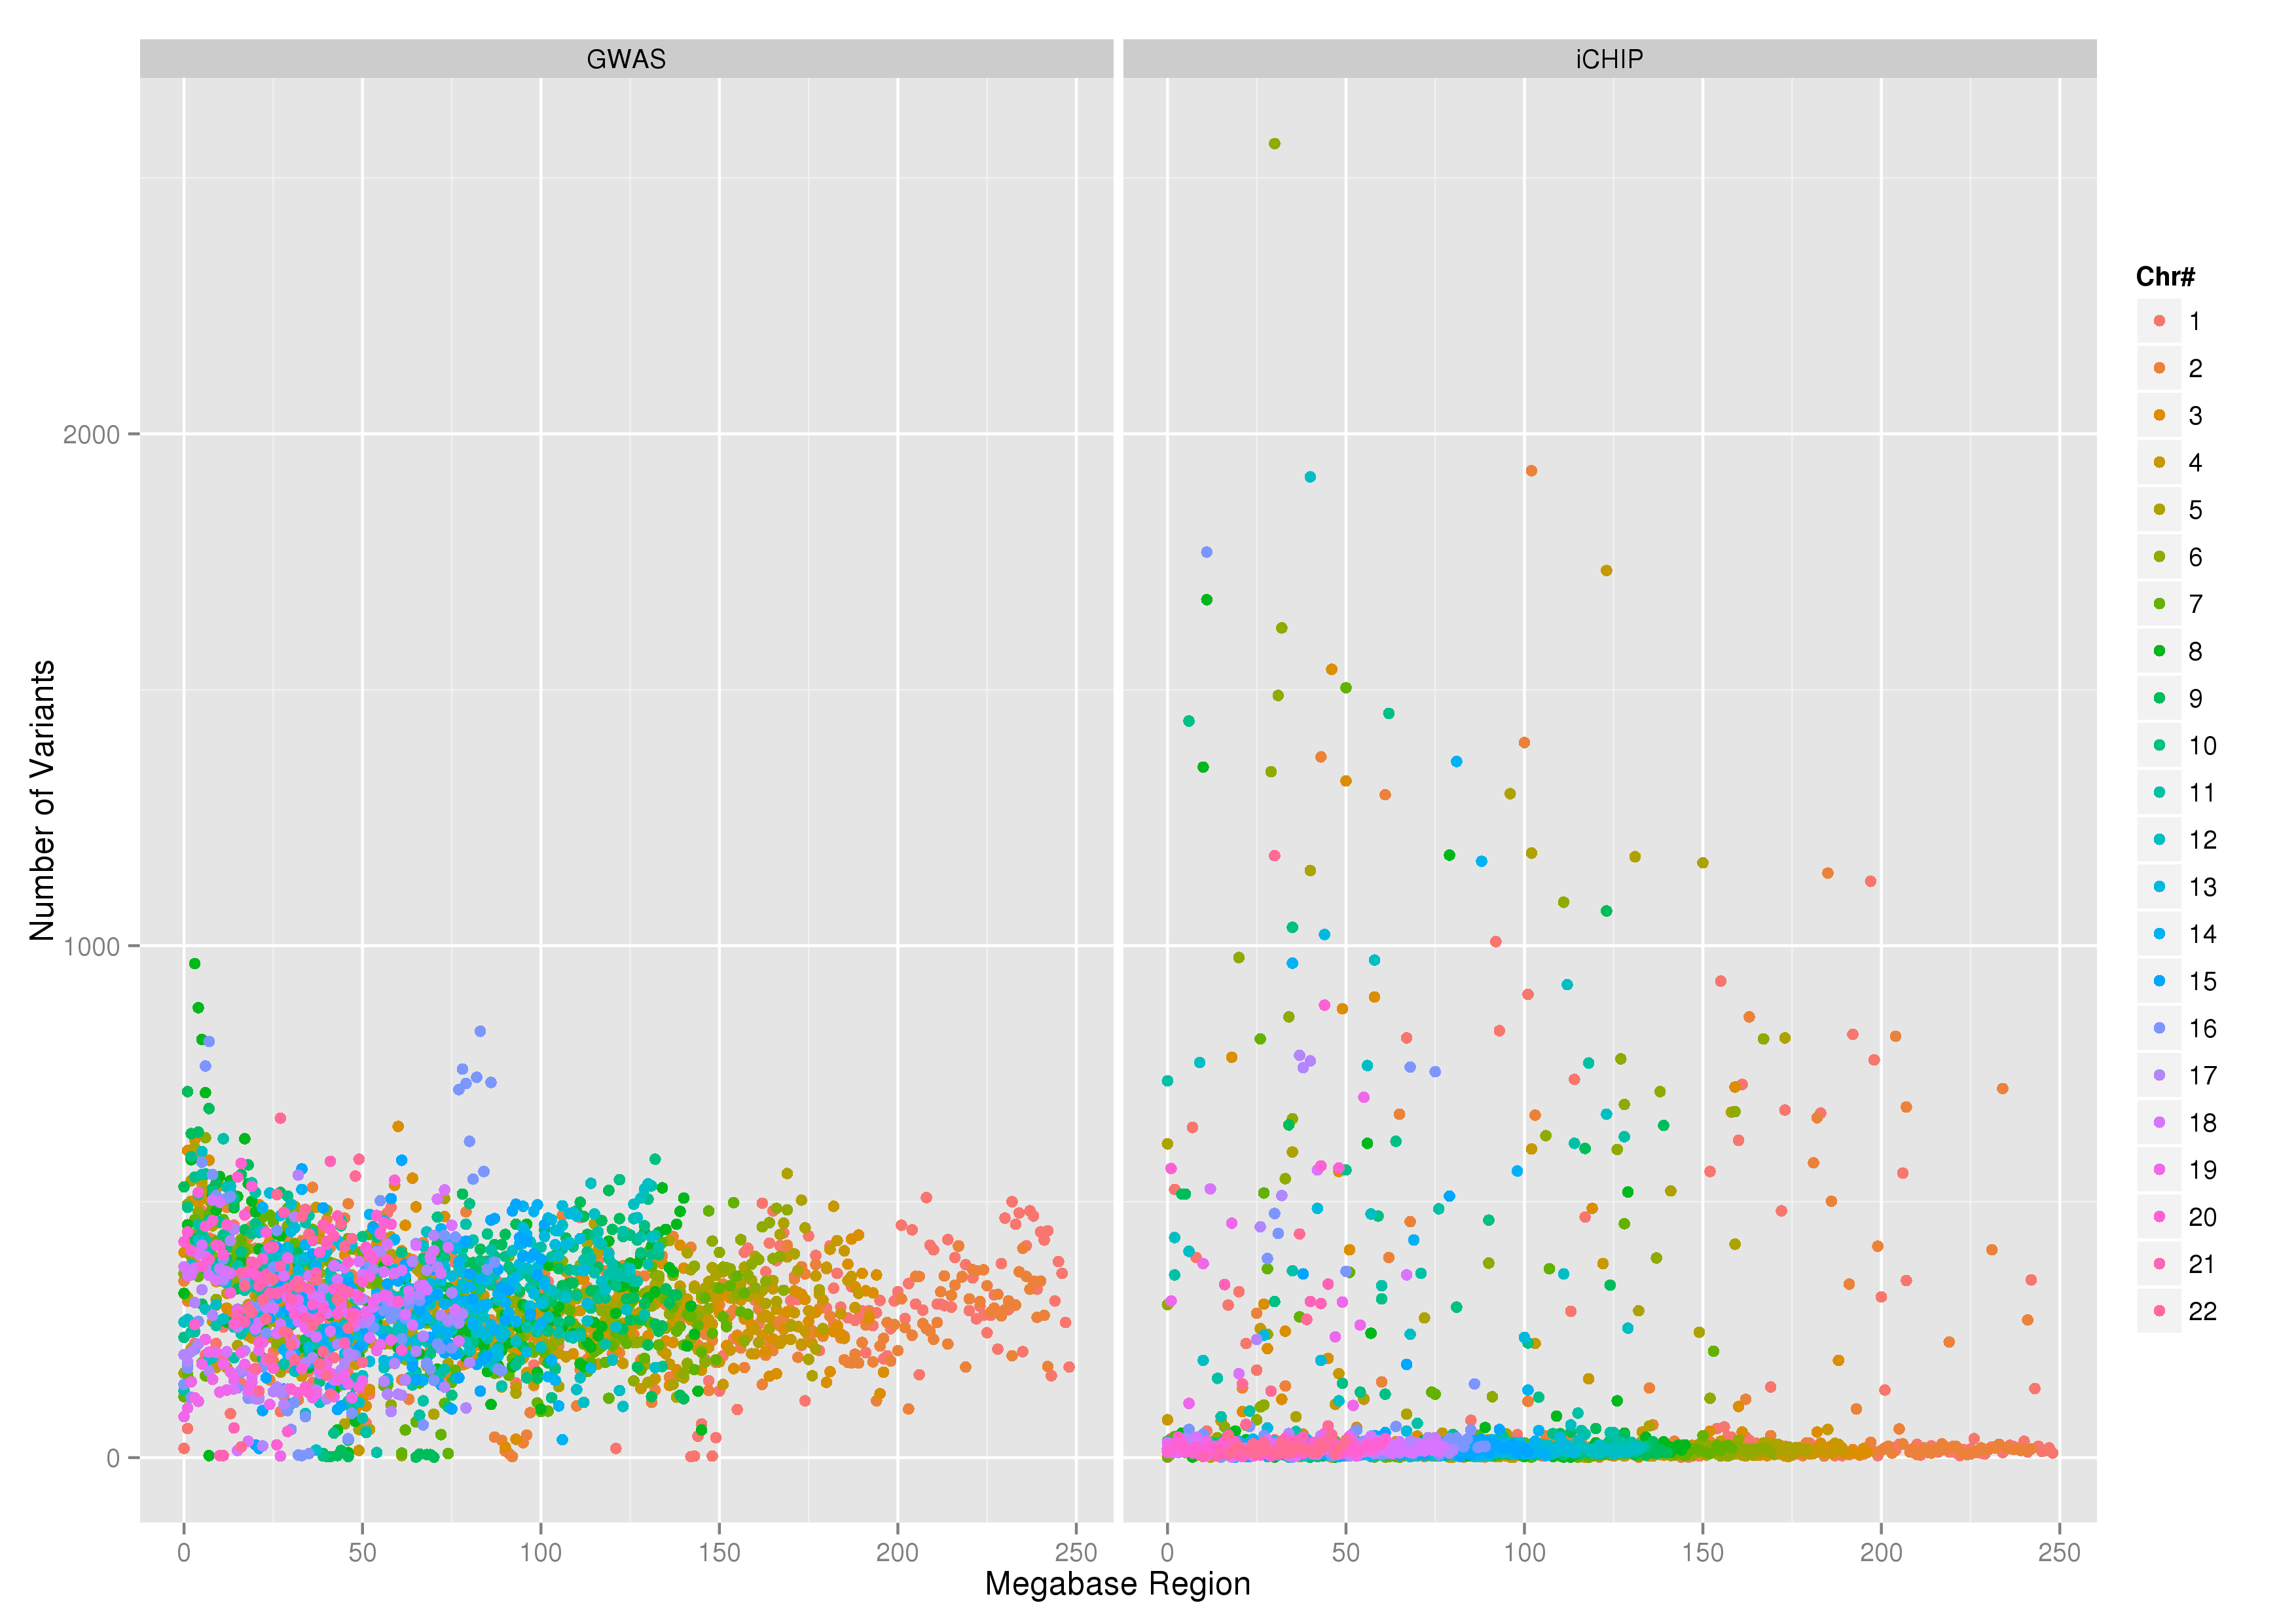
\includegraphics[width=1.0\textwidth]{megabase_plot}
    \caption[megabaseplot]{\textbf{Megabase Plot}: ...}
    \label{fig:megabaseplot}
\end{figure}


%%%%%%%%%%%%%%%%%%%%%%%%%%%%%%%%%%%%%%%%%%%%%%%%%%%%%%%%%%%%%%%%%%%%%%%%%%%%%%%
\chapter{Analysis Pipeline}
%TODO Explain experiment (reintroduce GWAS and SNP)

Following the extraction of the Goldilocks region for each of the samples... we
need to begin putting together the pipeline that would process the work for the
leave-one-out analysis...

%TODO Flow chart!

...involving generation of indexes for each sample
...execute the pipeline and withold one of the Goldilocks samples...
...using \textbf{samtools} to pileup the variants across all the samples
(excluding one of course) and then performing variant calling...
...must then compare the resulting VCF against the SNP VCF and calculate the
concordance to discover whether leaving out that particular sample has caused a
change in the accuracy of the variants called...


\section{Implementation}
\subsection{Region Extraction}

...regions extracted from IRODS
...difficulty gaining user access for both IRODS and "the farm"


\subsection{samtools index}
%TODO Cite index

...index extracted regions


\subsection{samtools mpileup}
%TODO Cite mpileup

Following extraction of the Goldilocks region for each full-genome sample, the
next stage is to use \textbf{samtools mpileup} to ...
...each of the various full genome samples we have for processing.  These files
are then summarised (and likelihoods are calculated) with samtools mpileup...

%TODO merge a list of what? Guess we've introduced BAM/VCF by now?
\textbf{samtools mpileup} is a rather intensive process especially when in a
scenario such as ours where there are thousands of input files, one for each of
the extracted regions. This not only places considerable strain on the cluster's
file system but is incredibly inefficient given the overhead of file handling.
As this pipeline will need to be executed once for each leave-one-out
experiment, it would be required to reduce the strain on the file server before
the job could be submitted. Usefully another member of the \textbf{samtools}
collection provides functionality to merge a list of given input files such as
those extracted Goldilocks regions.

% Needed -q long to submit to 48 hour queue instead of 12
\begin{minted}{bash}
    bsub -o ~/goldilocks/joblog/samtools_mpileup.%J.o -e
    ~/goldilocks/joblog/samtools_mpileup.%J.e -G hgi -J "samtools_mpileup"
    -M1000 -R "select[mem>1000] rusage[mem=1000]" bash -c 'samtools mpileup -b
    ../goldilocks-3:46000001-47000000.fofn -g -I -f
    /lustre/scratch113/resources/ref/Homo_sapiens/1000Genomes_hs37d5/hs37d5.fa >
    ~/goldilocks/all.withref.bcf'
\end{minted}


\subsection{samtools merge}

\subsubsection{Usage}
...undocumented feature to use a file of filenames... allowing more than two
files to be specified at a time...

\subsubsection{Memory Leak}

By default the LSF scheduler at the Sanger Institute will issue 100MB to any
submitted job. Given both the number of input files and their total size it was
anticipated that this merge job would require more memory. At the very least an
estimated 35kB for a 64-bit pointer to each input file and approximately 150MB
to house a 32kB buffer to read data from each file also. Yet executing the job
with 500MB caused the LSF scheduler to forceably terminate the process for
exceeding the maximum allocated memory limit.

Assuming that the intermediate structures for storing and sorting the input data
must have been greater than expected, the job's memory limit was generously
increased with the syntax demonstrated by Listing~\ref{list:lsf-memory} only to
meet the same fate, even when reserving 16GB of memory...

This is an absurd amount of memory even considering the vast input...
It appeared a memory leak had been discovered...
that drastically increases in severity as more files are provided as input,

%TODO Cite internal slides: Introduction to LSF at Sanger
% Farm Users Intro: Informatics System Group
\begin{listing}[H]
    \caption[lsf-memory]{: Flags required to raise job memory allocation}
    \label{list:lsf-memory}
    \begin{minted}[%mathescape,
                %linenos,
                gobble=8,
                frame=lines,
                framesep=2mm]{bash}
        bsub -R"select[mem>4000] rusage[mem=4000]" -M4000 ...
        #                 |                |        | Raise maximum job memory to 4000mb
        #                 |                | Pre-reserve 4000mb for job before execution
        #                 | Only run on a node with more than 4000mb memory
    \end{minted}
\end{listing}

...initial memory leak fixed by the author, several large variables not being
freed from memory...
...following this, further \textbf{samtools merge} jobs were submitted only to
also be repeatedly terminated by the LSF scheduler , this time for exceeding the
maximum execution time limit for the queue...

\subsubsection{Memory Leak in Test Harnesses}
...getline
...regcomp...

%TODO I
...other memory leaks still remained in the tests and wanting to brush up on
finding memory leaks with \textbf{valgrind}, I volunteered to locate and patch
these...

% https://github.com/samtools/samtools/pull/200
% http://valgrind.org/docs/manual/cl-manual.html

\begin{listing}[H]
    \caption[valgrind-regex]{: Example of \textbf{valgrind} locating a memory
        leak in one of the \textbf{samtools} test harnesses following the failure
        to release memory allocated to a compiled regular expression}
    \label{list:valgrind-regex}
    \begin{minted}[mathescape,
                %linenos,
                gobble=8,
                fontsize=\footnotesize,
                frame=lines,
                framesep=2mm]{bash}
        ==30464== 416 bytes in 1 blocks are indirectly lost in loss record 85 of 103
        ==30464==    at 0x4A082F7: realloc (in /usr/lib64/valgrind/vgpreload_memcheck-amd64-linux.so)
        ==30464==    by 0x3FBCCCA725: duplicate_node (in /usr/lib64/libc-2.17.so)
        ==30464==    by 0x3FBCCD3ADA: duplicate_node_closure (in /usr/lib64/libc-2.17.so)
        ==30464==    by 0x3FBCCD415A: calc_eclosure_iter (in /usr/lib64/libc-2.17.so)
        ==30464==    by 0x3FBCCD79F6: re_compile_internal (in /usr/lib64/libc-2.17.so)
        ==30464==    at 0x4A08121: calloc (in /usr/lib64/valgrind/vgpreload_memcheck-amd64-linux.so)
        ==30464==    by 0x3FBCCCCD88: create_cd_newstate (in /usr/lib64/libc-2.17.so)
        ==30464==    by 0x3FBCCCD506: re_acquire_state_context.constprop.41 (in /usr/lib64/libc-2.17.so)
        ==30464==    by 0x3FBCC2132E: build_trtable (in /usr/lib64/libc-2.17.so)
        ==30464==    by 0x3FBCCD3792: re_search_internal (in /usr/lib64/libc-2.17.so)
        ==30464==    by 0x3FBCCD8E94: regexec@@GLIBC_2.3.4 (in /usr/lib64/libc-2.17.so)
        ==30464==    by 0x40C6FA: check_test_2 (test_trans_tbl_init.c:124)
        ==30464==    by 0x402CC4: main (test_trans_tbl_init.c:348)
    \end{minted}
\end{listing}

\subsubsection{Poor Time Performance}
...submitting the same job to the "long" (48hr) and "basement" (essentially
unlimited) queues, it is clear that the job is taking an extraordinary length of
time to complete...

...during this time I took the opportunity to patch various memory leaks in the
test harnesses of both merge and split...

% http://kcachegrind.sourceforge.net/html/Home.html
% http://www.zlib.net/
valgrind, the tool I used to track down memory leaks in the test harnesses of
both samtools merge and samtools split actually consists of more than just
memcheck.

callgrind is a profiling tool that keeps track of a program’s call stack
history, a handy feature built in to some development environments such as
QtCreator.

Having constructed a modest test set of files to merge, I called samtools merge
from the command line, attaching callgrind and later imported the resulting
text file to QtCreator’s profiling tool to interpret the results (I usually use
KCacheGrind for this but I’ve been investigating QtCreator’s feature set for
reasons unrelated to this project), the result is immediately obvious -
millions of calls to functions in zlib; a free compression library.

% https://github.com/samtools/htslib/blob/develop/bgzf.c#L220
Further investigations using the QtCreator Analyze interface revealed that
these calls all boiled down to one line called not during the process of
deflating the input files (as I had expected) but actually during the
compression of the output!

\begin{figure}[htbp!]
    \centering
    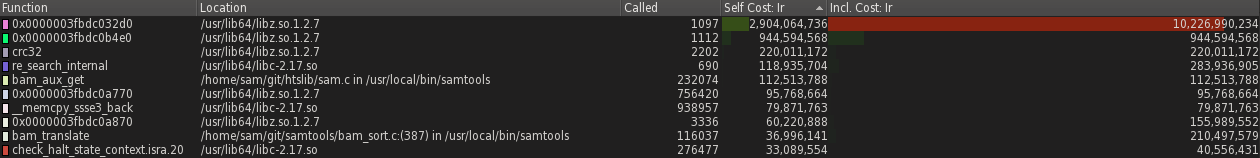
\includegraphics[width=1.0\textwidth]{callgrind_compressoutput_default}
    \caption[callgrind-default]{callgrind output following merge with default
    output compression}
    \label{fig:callgrind-default}
\end{figure}

\begin{figure}[htbp!]
    \centering
    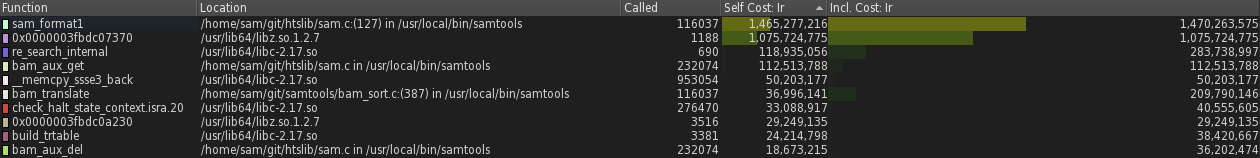
\includegraphics[width=1.0\textwidth]{callgrind_uncompressoutput}
    \caption[callgrind-uncompressed]{callgrind output following merge with
    uncompressed output}
    \label{fig:callgrind-uncompressed}
\end{figure}

% http://www.zlib.net/feldspar.html
Looking at a brief explanation of the deflate algorithm, it seems reasonable to
conclude the computational cost is rather asymmetric between compressing and
uncompressing - in that the effort is locating blocks to compress and in
comparison uncompressing is a reversible function on the known blocks.

Indeed, samtools merge specifies a -u option for uncompressed output and the
callgrind output (second image) indicates significantly less calls to zlib
functionality.

It remains to be seen whether this option will cut down the time needed for the
large merge job, perhaps this is merely a red herring and we’re yet to discover
the true speed trouble. In the meantime let’s see if sending this job to the
farm will work.


\subsubsection{The Red Herring}

% http://www.cs.utah.edu/dept/old/texinfo/as/gprof.html
... might be interesting to use gprof which is more
geared towards finding functions that spend all your execution time as opposed
to callgrind which I believe counts CPU instructions.

% http://paste.chippy.ch/woj.md
% https://github.com/samtools/htslib/blob/develop/sam.c#L1031
After re-compiling htslib and samtools with the -pg flag to enable such
profiling and executing the same previous merge command on the modest test set,
the output as parsed by gprof seems to indicate that the trouble lies with
bam\_aux\_get in htslib, with almost 50\% of the execution time being spent in
this particular function.

\begin{minted}[mathescape,
            %linenos,
            numbersep=5pt,
            %gobble=4,
            frame=lines,
            framesep=2mm]{c++}
    uint8_t *bam_aux_get(const bam1_t *b, const char tag[2])
    {
        uint8_t *s;
        int y = tag[0]<<8 | tag[1];
        s = bam_get_aux(b);
        while (s < b->data + b->l_data) {
            int x = (int)s[0]<<8 | s[1];
            s += 2;
            if (x == y) return s;
            s = skip_aux(s);
        }
        return 0;
    }
\end{minted}


% http://samtools.github.io/hts-specs/SAMv1.pdf
At a glance it seems that bam\_aux\_get receives a pointer to a BAM record and a
“tag”, an array of two characters representing an optional field as defined in
Section 1.5 of the SAM file spec.

The function then appears to fetch all these auxiliary tags and iterates over
each, comparing a transformation of that tag (x) to a pre-computed
transformation on the input tag (y).

% https://github.com/samtools/samtools/blob/2917ccdf34cd81b1327532b2db6e522fe871f054/bam_sort.c#L469
% https://github.com/samtools/samtools/blob/2917ccdf34cd81b1327532b2db6e522fe871f054/bam_sort.c#L484
% https://github.com/samtools/samtools/blob/2917ccdf34cd81b1327532b2db6e522fe871f054/bam_sort.c#L697
This would of course be inherently slow for files with many such tags;
especially given that the function is called twice for potentially each line in
a BAM file.


\subsubsection{The Plot Thickens}

% https://github.com/samtools/samtools/blob/2917ccdf34cd81b1327532b2db6e522fe871f054/bam_sort.c#L207
...as we increase the number of input files, the time taken to
read them in becomes non-linearly slower. Currently my money is on the seemingly
inefficient trans\_tbl\_init that appears to be called for each file, with the
current table of all previous files as an input...


\subsection{bcftools call}

%\citep{biostar:bcftools} https://www.biostars.org/p/96425/
...Unfortunately during the initial testing run of this step with all the
Goldilocks regions it was discovered that the output only included the standard
header information and not a single line for the variants themselves.

% http://samtools.github.io/bcftools/bcftools.html#call masked ref
...is because the piled up file was not generated with a corresponding reference
DNA sequence and so the REF (reference) column is set to N (an ambiguity code
which translates to ‘any base’).  bcftools call does have an -M flag to prevent
ignoring rows where the REF base is N (apparently called a "masked reference")
however this is currently causing a segmentation fault.  Having recompiled
htslib, samtools and bcftools I am now able to run bcftools call on my local
machine on some test data. I guess I’ll need to have someone recompile the
source for me on the cluster I’m using....



% ********************************** Back Matter *******************************
% ********************************** Bibliography ******************************
%\backmatter

\begin{spacing}{0.9}

% Bibliography style previews: http://nodonn.tipido.net/bibstyle.php

%\bibliographystyle{apalike}
%\bibliographystyle{plainnat} % use this to have URLs listed in References
\bibliographystyle{IEEEannot}

\cleardoublepage
\begin{multicols*}{2}
    \small{\bibliography{References/references}} % Path to your References.bib file
\end{multicols*}


\end{spacing}

% ********************************** Appendices ********************************

\begin{appendices} % Using appendices environment for more functunality

\chapter{Input Examples}

\section{BAMcheckR'd Example Output}
\label{app:bamcheckr}
\inputminted[fontsize=\scriptsize]{text}{Appendix1/example.bamcheck.SN.txt}

\section{auto\_qc Decision Matrix}
\label{app:aqc_matrix}
\inputminted[fontsize=\scriptsize]{text}{Appendix1/example.aqc.txt}


\end{appendices}

% *************************************** Index ********************************
%\printthesisindex % If index is present

\end{document}
